\documentclass[12pt,english]{article}
\usepackage{lmodern}
\linespread{1.05}
%\usepackage{mathpazo}
%\usepackage{mathptmx}
%\usepackage{utopia}
\usepackage{microtype}
\usepackage[section]{placeins}
\usepackage[T1]{fontenc}
\usepackage[latin9]{inputenc}
\usepackage[dvipsnames]{xcolor}
\usepackage{geometry}
\usepackage{amsthm}
\usepackage{amsfonts}
\usepackage{svg}
\usepackage{booktabs}
\usepackage{caption}
\usepackage{blindtext}
%\renewcommand{\arraystretch}{1.2}
\usepackage{multirow}
\usepackage{float}
\usepackage{rotating}

\usepackage{chngcntr}

% TikZ stuff

\usepackage{tikz}
\usepackage{mathdots}
\usepackage{yhmath}
\usepackage{cancel}
\usepackage{color}
\usepackage{siunitx}
\usepackage{array}
\usepackage{amssymb}
\usepackage{gensymb}
\usepackage{tabularx}
\usetikzlibrary{fadings}
\usetikzlibrary{patterns}
\usetikzlibrary{shadows.blur}

\usepackage[font=small]{caption}
%\usepackage[printfigures]{figcaps}
%\usepackage[nomarkers]{endfloat}


%\usepackage{caption}
%\captionsetup{justification=raggedright,singlelinecheck=false}

\usepackage{courier}
\usepackage{verbatim}
\usepackage[round]{natbib}
\bibliographystyle{plainnat}

\definecolor{red1}{RGB}{128,0,0}
%\geometry{verbose,tmargin=1.25in,bmargin=1.25in,lmargin=1.25in,rmargin=1.25in}
\geometry{verbose,tmargin=1in,bmargin=1in,lmargin=1in,rmargin=1in}
\usepackage{setspace}

\usepackage[colorlinks=true, linkcolor={red!70!black}, citecolor={blue!50!black}, urlcolor={blue!80!black}]{hyperref}
%\usepackage{esint}
\onehalfspacing
\usepackage{babel}
\usepackage{amsmath}
\usepackage{graphicx}

\theoremstyle{remark}
\newtheorem{remark}{Remark}
\begin{document}
	
\title{Endogenous Growth with Creative Destruction by Employee Spinouts}
\author{Nicolas Fernandez-Arias}
\date{\today \\ \small
	\href{https://drive.google.com/open?id=1NZCBFnkxug8qXWAZLTir6dEmIy9LuEBg}{Click here for most recent version}}
\maketitle



\begin{abstract}
	Knowledge spillovers have long been recognized as important drivers of aggregate productivity growth. For example, the flow of knowledge to startups founded by former employees, known as employee spinouts, is often credited with the emergence of Silicon Valley. However, when innovative efforts by incumbents create knowledge spillovers to competing firms, the effect of knowledge spillovers can be to discourage innovation by incumbent firms. The strength of this mechanism is particularly relevant to assessing the effect on growth of enforcing non-compete agreements, a policy question currently being discussed by several state legislatures. To explore and quantify this mechanism, I first esitmate the effect of corporate R\&D spending and subsequent formation of VC-funded startups by former employees in a micro dataset combining Compustat, the NBER-USPTO patent database, and Venture Source data on VC-funded spinouts. Interpreting the estimates as causal, I find that approximately 25\% of spinouts in the data resulted from R\&D expenditures of previous employees, 45\% of which are in the same 4-digit NAICS industry as the parent firm. To quantify the importance of this mechanism for productivity growth, I develop a model of endogenous growth with creative destruction by employee spinouts. The model proceeds from the hypothesis that, absent NCAs, R\&D projects by incumbents lead to formation of employee spinouts which do not maximize the joint surplus of the incumbent-employee pair. This can result from asymmetric information or disagreement between the worker and the firm concerning the value of the idea; I leave this unmodeled for tractability. Spinouts implement ideas that otherwise would not be implemented, so easier spinout formation expands the production possibilities frontier of the economy. However, the possibility of future spinouts which do not maximize joint surplus discourages incumbent R\&D. In addition, the model exhibits an "escape competition" effect: the stock of spinouts encourages incumbent R\&D because successfully innovating increases technological distance and hence the duration of the its monopoly. The net effect is that for some parameters the rate of spinout formation has a non-monotonic effect on steady state growth and welfare. Relatedly, enforcing non-compete agreements can increase or decrease both growth and welfare. To impose discipline on these parameters, I calibrate the model. For some parameter values, expanding the production possibilities frontier by increasing the using my estimates from the micro data, aggregate moments and parameters from the literature. I use the model to study the effect on steady state growth and welfare of increasing or decreasing the enforceability of non-competes, as well as other policies such as R\&D subsidies and startup subsidies. Since the identification of parameters is not ideal, I close with a discussion of how the implications of the model depend on the key parameters, and how they might be estimated in future work. 
	
\end{abstract}

\tableofcontents

\section{Introduction}


Silicon Valley (SV) is widely viewed as a highly innovative region. This can be seen readily in the data: for example, labor productivity growth in the MSA containing SV averaged 2.72\% from 1978 to 2015, compared to an average of about 2\% for the whole country during that time period. This difference in growth rates implies a 30\% increase in the level of productivity over the time period, which likely underestimates the contribution to aggregate labor productivity growth for several reasons. \footnote{See \cite{parilla_understanding_2017}. Further, the employment growth rate exceeded the national average during this time period, increasing the contribution to aggregate labor productivity growth. Even more importantly, labor productivity growth in SV has been centered on ICT-producing firms, whose output contributes heavily to labor productivity growth in other industries. \cite{jorgenson_retrospective_2008} attributes nearly half of labor productivity growth from 1973-2006 (and more 60\% from 1995-2000) to ICT. Consistent with this, the appendix of  \cite{parilla_understanding_2017} reports that labor productivity growth peaked at almost 5\% annualized in the MSA containing SV from the years 1994-2005.} The literature has argued for the importance of employee mobility and entrepreneurship in the region, with a particularly important part played by \textit{employee spinouts}: firms founded by former employees in the same or related industries as the former employer. \footnote{See \cite{saxenian_regional_1994}, \cite{gilson_legal_1999}, \cite{fallick_job-hopping_2006}, \cite{franco_covenants_2008}.} \footnote{This is different from a "spinoff", which is a division of a firm that the firm itself decides to sell. The early literature uses these terms interchangeably, but the more recent literature has settled on the term "spinout" for entrepreneurship initiated by the employee.} As an anecdotal illustration, Figure \ref{fairchild_spinouts} shows the many direct and indirect spinouts of Fairchild Semiconductor, one of the first leading semiconductor firms of SV -- itself a spinout of Shockley Laboratories, another semiconductor firm. Although Fairchild was founded in the 1950s, its list of spinouts includes some of the most well-known modern firms in SV, such as Intel and AMD. 

\begin{figure}	\phantomsection
	\center
	\includegraphics[scale = 0.77]{../figures/fairchildren_early.png}
	\caption{Direct and indirect spinouts of Fairchild Semiconductor}
	\label{fairchild_spinouts}
\end{figure}



In turn, the literature has argued that SV's high employee mobility and entrepreneurship is due in large part to California's radical prohibition of \textit{non-compete agreements} (NCAs). Such contracts prevent departing employees from joining or founding competing firms for a span of time (usually six months to two years) and often in a certain geographical region. However, theory is ambiguous about the relationship between NCA enforcement and innovation. The limited excludability of knowledge means the returns to investment cannot be fully appropriated, reducing investments in knowledge. If NCA enforcement reduces the formation of spinouts, incumbent firms can better appropriate the returns of knowledge investments, increasing incentives to innovate. Viewed this way, NCAs are similar to patents, which also create incentives while reducing competition and knowledge spillovers.

Of course, the specific cause of SV's rise is difficult to ascertain. Nevertheless, the preceding question motivates the general question of what effect spinout entrepreneurship -- and in particular enforceability of non-competes -- has on innovation and labor productivity growth. In particular it is essential to understand the answer to this question to properly assess the role of knowledge spillovers in productivity growth. This paper attempts to take a step towards answering this question.

First, I assemble a dataset of parent firms and startups founded by their employees by combining Compustat data on publicly traded firms and Venture Source data on VC-funded startups and their founders. While the Venture Source data has limitations, it is the only dataset of startups with information on the most recent employer of the startup's key employees. Matching these data is somewhat challenging since there are no company identifiers across datasets: the match must be done by name only. This is non-trivial since companies go by different names. I solve this problem by using string matching techniques (e.g., regular expressions), Compsutat data on subsidiaries and finally the merchant-mapper tool by Alternative Data Group, a startup that links credit card transactions data to firms using machine learning (itself a spinout of 1010 Data). I define a startup as a spinout if its CEO, CTO, President, Chairman or Founder (1) was most recently employed at a firm in Compustat and (2) joined the startup in its first three years. Using this definition, I identify approximately 10,000 employee spinouts. Further, I also match these data to patent data using the NBER-USPTO patent database. 

Using this dataset, I document the relationship between R\&D spending at public firms and subsequent spinout formation by their employees. A simple regression of number of employee spinouts on lagged R\&D spending suffers from omitted variable bias, as factors such as changes in demand or changes in technological investment opportunities likely affect both variables in the same direction. To control for this, I use firm, state-year, NAICS 4 digit industry-year, and firm age fixed effects, as well as firm-specific controls, such as citation-weighted patents. Based on this estimate, R\&D accounted for approximately 25\% of the spinouts in my sample, and 50\% of these R\&D-induced spinouts are in the same NAICS 4-digit industry as one of their parent firms. Employee spinouts are also 50\% more likely to be eventually acquired or IPO. For the purposes of my subsequent analysis, I interpret this accounting decomposition as causal. 

I next develop a model of endogenous growth in which R\&D leads to formation of spinouts by employees and study its balanced growth path. The model takes as given that, absent NCAs, R\&D projects by incumbents lead to formation of employee spinouts which do not maximize the joint surplus of the incumbent-employee pair. This failure in the "market for ideas" can result from at least three frictions: private information concerning the quality of the idea, disagreements between the employee and the employer concerning the idea's quality, and the lack of commitment power on the part of the employee (i.e., the employee cannot commit not to implement the idea even after notionally selling it to his employer).\footnote{I leave these considerations unmodeled for the sake of tractability, but not because they are not important. And, crucially, the economic forces that generate a "need" for non-compete agreements -- the fact that the knowledge transfer of within-industry spinout ideas from employer to employee is "leaky" -- can help revive the market for ideas, by creating a gap in the employer / employee value of the idea (taking into account business stealing effects of spinouts). If there are no property rights on ideas, this logic can still be valid (in a weakened way) if the firm can hire the employee to "do nothing": provided the worker's outside option (i.e. other than the idea) is not too valuable, this is only a somewhat expensive way of creating a de-facto non-compete contract. In future work, I plan to address these issues.} 

Because spinouts implement ideas that otherwise would not be implemented, reducing barriers to spinout formation expands the production possibilities frontier of the economy. Still, the effect on welfare is not clear. In the laissez-faire equilibrium, incumbent firms' private return from innovation is below its social return, due to knowledge spillovers and the effect of increased product-market competition on consumer welfare (not present in the current model). However, knowledge spillovers to future competitors via spinouts are a particularly costly way to obtain these benefits, since they sharply reduce the return to the production of knowledge. On the other hand, knowledge spillovers to future competitors of \textit{other firms} reduce the pre- and post-innovation rents of these firms, reducing their effect on incentives to innovate. Provided that (1) NCAs increase the incentive to innovate (see the next paragraph) and (2) knowledge spillovers to different industries are sufficiently frequent and socially valuable, their use can have a beneficial effect: the loss of knowledge spillovers within-industry can be offset by increased innovation incentives of incumbents and increased knowledge spillovers to other industries.\footnote{In fact, even when all spinouts are WSOs, growth and welfare can be decreased for sufficiently high rates of spinout formation. However, this requires assumptions that R\&D leads to competition that is much too strong than is consistent with the data on spinout formation.}

One caveat is the "escape competition" effect, whereby the stock of WSO-spinouts attempting creative destruction of the parent encourages incumbent R\&D, because successfully innovating increases the expected duration of the incumbent's monopoly.

Finally, I use the model to conduct a quantitative analysis of the growth and welfare consequences of non-compete enforceability. To impose discipline on the model, I calibrate it using my estimates from the micro data, aggregate moments and parameters from the literature. I use the model to study the effect on steady state growth and welfare of increasing or decreasing the enforceability of non-competes, as well as other policies such as R\&D subsidies and startup subsidies. Since the identification of parameters is not ideal, I close with a discussion of how the implications of the model depend on the key parameters, and how they might be estimated in future work. 

\paragraph{Related literature}

Some work has attempted to answer this question directly using empirical methods. Papers in this literature have typically used either cross-sectional and/or longitudinal variation in the state-level enforcement of non-competes.\footnote{Sometimes this variation is argued to be exogenous, either due to legislative error as in \cite{marx_mobility_2009} and \cite{marx_regional_2015}, or due to unexpected judicial precedent as in \cite{jeffers_impact_2018}. Often there is a control industry that is believed to be unaffected by the variation in CNC enforcement policy (e.g. law firms are typically exempt from CNC restrictions).} The results are inconclusive and suggest an important tradeoff between entry of spinouts and investment by incumbent firms. \cite{stuart_liquidity_2003} find more local  entrepreneurship in response to local IPO (a "liquidity event") in regions not enforcing CNCs. \cite{marx_mobility_2009} finds that inventor mobility declines in response to an increase in non-compete enforcement. \cite{samila_venture_2010} finds that an increase in VC funding supply increases entrepreneurship more in states without non-compete restrictions, using an IV design. \cite{garmaise_ties_2011} finds that, in states where CNCs are more enforceable, managers are less mobile, have lower compensation, and invest less in their human capital, to the point of offsetting increased investments by the firm. On the other hand, \cite{conti_non-competition_2014} finds evidence that non-compete enforceability leads to incumbent firms pursuing riskier R\&D projects. \cite{colombo_does_2013} finds evidence that easier spinout formation -- proxied by access to finance -- leads to a reduction in incumbent firm knowledge investments.  Most recently, \cite{jeffers_impact_2018} uses data on influential state-level court precedents matched with LinkedIn data and finds that enforcement indeed reduces spinout formation while increasing capital investment by incumbent firms. Finally, \cite{marx_regional_2015} finds that CNC enforcement leads to inventor mobility out of the state, suggesting that differences in outcomes could be in part due to reallocation. 

Theoretical work has also explored this question. As mentioned previously, \cite{franco_spin-outs:_2006} develops a model in which employees learn from their employers and use this knowledge to form spinouts. They emphasize the "paying for knowledge" effect, whereby employees implicitly pay for the knowledge they take from the parent firm through lower equilibrium wages. Importantly, they assume spinout firms do not steal business from their parents: the only effect of a spinout on the parent firm is a reduction in the price of the output good, which the parent firm is assumed not to take into account. This, combined with the "paying for knowledge" mechanism, ensures that the competitive equilibrium allocation is Pareto efficient, even without resorting to elaborate labor contracts.

\cite{franco_covenants_2008} studies a two-period, two-region model with employee spinouts in which the region which does not enforce CNCs initially lags but eventually overtakes the region in which CNCs are enforced. In the first period, entry is more valuable in the enforcing region. But in the second period, spinouts enter in the non-enforcing region, there is Cournot competition with parent firms in the product market, and output increases relative to the enforcing region. The analysis emphasizes how asymmetric information about whether an employee has learned leads some firms in the non-enforcing region to allow spinouts (assuming firms cannot commit to wage backloading). This can be taken as a rough microfoundation of my assumption that labor contracts are "simple" in  a non-enforcing region: just a wage, with no attempts at retention in the case of learning. They do not consider long-run growth implications, and use a two period model. Spinouts do not worry about spinouts of their own. R\&D is not present - only entry in the first period leads to a certain chance of spinout formation in the second period. 

\cite{shi_restrictions_2018} uses a rich model of contracting disciplined by data on executive non-compete contracts to study the effect of non-competes on executive mobility and firm investment. She finds that the optimal policy is to somewhat restrict the permitted duration of CNCs. Her approach allows her to study the optimal contracting problem in more detail than in mine. However, she is mainly interested in poaching, which involves an attempt to extract a payout from the poaching firm, while I am interested in spinouts. Also, her calibration relies heavily on matching the response of firm investment to the presence of a CNC in the manager's contract. However, she uses capital investment rather than investment in knowledge. This leads her to estimate an R\&D elasticity such that non-competes do not do much to increase the incentives for firm investment. However, I am interested in long-run growth, which is driven by investments in knowledge (in the data, R\&D not capex).

\cite{baslandze_spinout_2019}, the study closest to this paper, studies the effect of spinout entrepreneurship on entry and growth. Baslandze's analysis concludes that the optimal enforcement of non-competes is zero. However, in her framework, spinouts do not steal business from the parent firm, instead entering into a different product line. The harm to the parent firm results from the additional assumption that the parent firm's technology gap -- relative to potential entrants in its own product-line -- drops to zero upon spinout formation. This is modeled as other firms "catching up" technologically to the incumbent, although it is interpreted as the loss of match-specific productivity. In other words, the knowledge of the firm is fully embodied in its R\&D manager. My paper focuses instead on creative destruction of the parent firm using knowledge that is embodied in the firm but can be used simultaneously by the employee in a spinout.  More importantly, in her analysis, higher non-compete enforcement is modeled as a higher cost of spinout formation. This is unsatisfactory because it precludes the possibility that bilaterally efficient spinouts will be allowed even in CNC enforcing regions. 

Most recently, Babina \& Howell 2019, finds a relationship between corporate R\&D spending and employee spinout formation. They find a positive result.\footnote{Their study is simultaneous to this one and complementary to it. They use LEHD data to identify spinouts via the previous employment of the highest paid employee of entering firms. Due to their higher sample size (they have observations at the establishment level), they are able to leverage instruments for R\&D spending based on \cite{bloom_identifying_2013}, which do not have sufficient power for my setting.}

(transition into literature review, in progress)

This paper relates to several existing branches of the literature. 

First, there is a long empirical literature on the innovative activities of firms; see \cite{cohen_fifty_2010} for an excellent survey.

Literature on spinoffs and knowledge appropration: \cite{anton_expropriation_1994}, \cite{anton_start-ups_1995}, \cite{franco_covenants_2008}, \cite{klepper_entry_2005}, \cite{klette_innovating_2004}, \cite{chatterjee_spinoffs_2012}

Literature on endogenous growth: \cite{grossman_quality_1991}, \cite{romer_increasing_1986}, \cite{aghion_model_1992}

Literature on non-competes: \cite{saxenian_regional_1994}, \cite{gilson_legal_1999}, \cite{jeffers_impact_2018}, \cite{marx_mobility_2009}, \cite{marx_regional_2015}, \cite{starr_noncompetes_2019}

Literature on the relationship between competition and innovation: \cite{aghion_competition_2005}


\section{Empirics}

\subsection{Data}

\paragraph{Venture Source}

Venture Source (VS) is a proprietary dataset containing information on venture capital (VC) firms and VC-funded startups. I use a subsample of the data for US-based startups founded between 1986 and 2008 which contain information on their founding year. The data cover 23,434 startups, 89,382 financing rounds, and 297,119 individual-firm pairs. For each financing round, the data contain information on valuation, amount raised, and status of the business at the time of the round -- employment, revenue, net income, burn rate -- albeit with substantial missing data. Crucially for this analysis, the data contain employment biographies for each startup's founders and key employees (C-level, high-ranking executives and managers) and board members. Some summary information about the dataset is contained in \autoref{table:VS_summaryTable}. The dataset is described in detail in \cite{kaplan_how_2002} and \cite{kaplan_venture_2016}. 

\paragraph{Compustat}

Compustat is a comprehensive database of fundamental financial and market information on publicly traded companies. The main part of this study considers a subsample consisting of all firms headquartered in the United States in operation at any point between 1986 and 2006, consisting of 20,534 firms. The Compustat data has information on R\&D expenditures at the firm-year level as well as time-varying firm controls.

\paragraph{NBER USPTO patent data}

The NBER-USPTO database contains comprehensive information on all patents granted in the United States from 1976 to 2006, and is linked to Compustat. I consider the subsample of patents assigned to US firms, consisting of 1,457,136 patents. 

\subsection{Constructing dataset on employee spinouts}

\subsubsection{Defining a ``founder''}

I consider a \textbf{founder} to be an individual who joined a startup in its first three years. When information on the individual's date of joining the startup is missing, I impute it as the founding date of the startup. I also conduct robustness exercises where I exclude these individual-startup observations. 

As noted above, many such founders do not have roles directly related to the operation of the firm. The breakdown of the 20 most frequent titles is shown in \autoref{table:VS_titlesSummaryTable}. Nearly 35\% of founders are outside board members. I define \textbf{key founders} as founders with the title Founder, Chief, CEO, CTO or President. Similarly, \textbf{executive founders} include key founders as well as CFO, COO, CSO (Chief Science Offier), CIO (Chief Information Officer), Chairman, Executive Vice President, Managing Director or Manager. 

Finally, I define \textbf{techincal founders} to be founders with the title Founder, CTO, CSO, CIO or Scientific Advisor. This category reflects the study's focus on knowledge spillovers through employee mobility.

% latex table generated in R 3.6.3 by xtable 1.8-4 package
% Tue Jul  7 15:40:11 2020
\begin{table}[!htb]
\centering
\begingroup\footnotesize
\begin{tabular}{rll}
  \toprule
Title & Individuals & Percentage \\ 
  \midrule
Board member (outsider) & 103367 & 34.6 \\ 
  Vice President & 59149 & 19.8 \\ 
  Chief Executive Officer & 24230 & 8.1 \\ 
  Chief Technology Officer & 13971 & 4.7 \\ 
  Chief Financial Officer & 11621 & 3.9 \\ 
  Director & 10988 & 3.7 \\ 
  Chief & 10846 & 3.6 \\ 
  President \& CEO & 9088 & 3.0 \\ 
  Senior Vice President & 8700 & 2.9 \\ 
  Founder & 8471 & 2.8 \\ 
  Chief Operating Officer & 6777 & 2.3 \\ 
  President & 5441 & 1.8 \\ 
  Chairman & 5029 & 1.7 \\ 
  Executive Vice President & 4920 & 1.6 \\ 
  Chairman \& CEO & 2755 & 0.9 \\ 
  Manager & 2357 & 0.8 \\ 
  Chief Scientific Officer & 1461 & 0.5 \\ 
  Controller & 1137 & 0.4 \\ 
  President \& COO & 1134 & 0.4 \\ 
  General Counsel & 1056 & 0.4 \\ 
   \bottomrule
\end{tabular}
\endgroup
\caption{Top 20 most frequent titles among founders in VS data.} 
\label{table:VS_titlesSummaryTable}
\end{table}


\subsubsection{Finding most recent employer}

In order to relate the activities of employers to the entrepreneurship behavior of their employees, I link the Compustat data to the VS data using information in employee biographies. Because VS biographies are text fields, this requires matching entries by name to firm names in Compustat.  

The VS biographical data comes in a structured format, allowing parsing by regular expressions. Each prior job is represented in the format ``<position>, <employer>'' and different jobs are separated by ``;''. Job spells can be easily separated by splitting the string on the character ``;''. It is slightly more involved to separate positions from employer. It is not sufficient to simply separate on the right-most character ``,'' as <employer> can contain ``,''. However, in almost all cases, <employer> contains at most one ``,'' (e.g., in ``Microsoft, Inc.''), and in virtually all of these cases, the comma precedes one of a few strings (e.g. ``LLC'',``Inc'',``Corp''). Hence, I use a two-pass approach: first I split on the last ``,''; for employers that end up consisting only of corporate structure (e.g., ``LLC'', etc.), I split on the penultimate ``,'' instead. 

The above procedure yields a dataset containing, for each individual, his or her 15 previous positions and employers. However, because an individual can take various jobs over the years at an individual startup, there are individuals whose most recent employer coincides with their startup. I exclude these cases by comparing the previous employer with the \texttt{EntityName} text field. Because these are both text fields with potentially different formatting, this entails two steps. First, I bring both fields to a common format, eliminating endings such as ``Inc.'', ``Corp.'' etc which may vary across them, and converting to lower case. I then exclude observations where the strings either exactly coincide or one contains the other. 

The results of this procedure are summarized in \autoref{table:VS_previousEmployersSummaryTable}. The top previous employers include several well-known technology firms such as Microsoft, IBM, Google, and Oracle. However, notice that many of the top previous employers are VC firms (e.g., New Enterprise Associates, Sequoia Capital, Kleiner Perkins), and the top employer is the unaffiliated category "Individual Investor." This is largely because many of the individuals affiliated with startups are investors turned board members: about 33\% of the individual-startup observations are outside board members, As my focus is on the flow of knowledge from previous employers to new startups, I will later restrict attention to individuals with knowledge-related and/or executive titles. Finally, notice that Stanford University is also listed in the top 20. Several other prominent research universities are also in the top 50. 

% latex table generated in R 3.4.4 by xtable 1.8-4 package
% Thu Feb  6 14:38:23 2020
\begin{table}[!htb]
\centering
\begingroup\footnotesize
\begin{tabular}{rlrll}
  \toprule
Employer & Count & Position & Count & Percentage \\ 
  \midrule
Individual Investor & 1115 & Board Member, Institutional Investor & 38527 & 14.2 \\ 
  Microsoft & 938 & Executive & 19617 & 7.2 \\ 
  Google & 780 & CEO & 9681 & 3.6 \\ 
  IBM & 773 & President \& CEO & 6871 & 2.5 \\ 
  Cisco Systems & 690 & CFO & 6567 & 2.4 \\ 
  Oracle & 602 & President & 5741 & 2.1 \\ 
  New Enterprise Associates & 565 & Founder & 4964 & 1.8 \\ 
  AT\&T & 466 & Cofounder & 3884 & 1.4 \\ 
  Verizon & 443 & Partner & 3757 & 1.4 \\ 
  Sun Microsystems & 402 & CTO & 3491 & 1.3 \\ 
  Intel & 389 & Managing Director & 3381 & 1.2 \\ 
  Hewlett-Packard & 386 & VP & 3365 & 1.2 \\ 
  Sequoia Capital & 384 & COO & 2445 & 0.9 \\ 
  Venrock & 342 & Board Member, Outsider & 2260 & 0.8 \\ 
  Kleiner Perkins Caufield \& Byers & 334 & Director & 2221 & 0.8 \\ 
  Mayfield Fund & 310 & Chairman \& CEO & 2147 & 0.8 \\ 
  McKinsey \& & 307 & Founder \& CEO & 2091 & 0.8 \\ 
  Bessemer Venture Partners & 305 & Chairman & 2086 & 0.8 \\ 
  Stanford University & 298 & Principal & 1836 & 0.7 \\ 
  Ernst \& Young & 275 & VP, Marketing & 1785 & 0.7 \\ 
   \bottomrule
\end{tabular}
\endgroup
\caption{Top 20 previous employers and previous positions for founders in VS data.} 
\label{table:VS_previousEmployersSummaryTable}
\end{table}


\subsubsection{Linking to Compustat}

The data on prior employers is matched to the variable \texttt{conml} in Compustat. To do this, first I standardize names as before, using regular expressions to trim e.g. ``Inc.", ``Corp.'' and variants thereof from each entry and converting to lower case. I look for exact matches to previous employers in the VS data. For previous employers in VS that do not match with any names in Compustat, I check against the business segment names, available from the Compustat Segments database. 

\paragraph{AltDG}
[Alt DG - need to decide if doing it and try robustness later, but there are substantial issues - for now leave out]


\subsubsection{Defining WSOs}

This study emphasizes the importance of competition between spinouts and their parent firms. The best measure I have for the product market of publicly traded firms is their self reported NAICS code. While VS does not contain NAICS classifications for its startups, it does document their industry using a classification that, for the most part, coincides with NAICS 4 or 5 digit categories. I manually construct a crosswalk between the two classification schemes and use this to assign 4-digit NAICS codes to startups in VS.\footnote{An alternative would be to us VS's "Competition" variable, which documents directly the competitors of the startup observation. However, only 20\% of startups have this variable filled in: 30\% in the 90s, but dropping to around 10\% by the end of the sample.} Then, I classify a founder-startup observation as a \textbf{$i$-digit within-industry spinout (WSOi)} whenever the startup is in the same $i$-digit NAICS category as its parent. 

\subsubsection{Evaluating the match}

\autoref{table:GStable_founder2} documents the quality of this match for \textbf{key founders} on the subset of startups with at least one key founder. It corresponds roughly to Table 1 of \cite{gompers_entrepreneurial_2005}.\footnote{The numbers are different. I find a similar number of founders from public companies, but a substantially smaller fraction. I suspect this is due to startups being added to the data retroactively since the time of that article \textbf{[ask VS]}.} About 20\% of key founders have previous employers that match to a public firm in Compustat. In turn, about 35\% of these come from the same 4-digit NAICS codes. The numbers for different definitions of founders are similar. 

\autoref{figure:industry_row_heatmap_naics2_founder2} and \autoref{figure:industry_column_heatmap_naics2_founder2} document the joint distribution of parent industry and child industry, defined by 2-digit NAICS codes.\footnote{In the appendix, figures \ref{figure:industry_row_heatmap_naics3_founder2} and \ref{figure:industry_column_heatmap_naics3_founder2} show the same picture with 3-digit NAICS codes.} The raw joint distribution is too heavily concentrated to be easily visualized in this way, so instead I show the distribution of child industry (parent industry) conditional on parent industry (child industry), displayed in \autoref{figure:industry_row_heatmap_naics2_founder2} (\autoref{figure:industry_column_heatmap_naics2_founder2}). The dark diagonal lines in both figures reflects the prevalence of WSOs. In \autoref{figure:industry_row_heatmap_naics2_founder2}, the dark vertical line at column 51 (Information) indicates that parent firms of all industries tend to spawn spinouts in that industry. Similar dark regions appear at columns 54 (Professional, Scientific and Technical Services), and 32 and 33 (Manufacturing). In \autoref{figure:industry_column_heatmap_naics2_founder2}, the dark horizontal lines at 51 and to a lesser extend 32, 33, 52 and 54 indicate that child firms of all industries tend to have founders from those industries.

As an aside, Figures \ref{figure:state_row_heatmap_founder2} and \ref{figure:state_column_heatmap_founder2} visualize the joint distribution of parent state and child state. Again, the dark lines along the diagonal reflect that spinouts tend to be geographically proximate to their parent firms. The dark vertical line in \ref{figure:state_row_heatmap_founder2} at the column labeled ``CA'' indicates that spinouts from all states are likely to occur in California. Similarly, the dark horizontal lines at the rows labeled ``CA'' AND ``NY'' show that there are many states whose spinouts are likely to have their root in California or New York. 

\subsection{Characteristics of spinouts and WSOs}\label{subsec:Char_of_spinouts_and_WSOs}

In this section I document some differences in fundamentals between ordinary startups, employee spinouts, and WSOs. To do so, I make use of the VS data on employment, valuation, revenue and exits (out of business vs. acquisitions and IPOs). Throughout the main text, I use the \textbf{key founder} definition of founder. 

\paragraph{Defining spinouts}

I classify a startup as a spinout when at least 30\% of its founder-startup observations have a most recent employer in the Compustat database. Similarly, I classify a spinout as a WSOi whenever at least 30\% of its founder-startup observations were most recently employed a Compustat firm in the same $i$-digit NAICS industry.


\paragraph{Imputing employment, valuation and revenue} When recorded, information on employment and valuation is available at each deal. 50\% of deals have data on current employment and 25\% of deals have data on post-money valuation. 85\% (40\%) of startups have at least one non-missing employment (valuation) observation. I expand this dataset to a dataset with observations for every startup-year in between the founding date and the last date the startup appears in VS. This is either the last deal date or, when available, the date registered in the \texttt{OwnerStatDate} variable. 

In the resulting dataset, 22\% (11\%) of startup-years have information on employment (valuation). Conditional on the startup having any employment (valuation) information, 25\% (24\%) of startup-years have data on employment (valuation). 

Revenue information is available in an auxiliary dataset for certain startup-year combinations. 24\% of startups have some information on revenue. I merge this with the employment and revenue dataset by startup and year. In the resulting dataset, 7\% of startup-years have information on revenue. Conditional on the startup having any revenue information, 20\% of startup-years have revenue data.

\textbf{Is it worth it to do this?} To be sure, there is substantial missing data. Rather than treat the startup-years with missing data as unusable observations, I use an imputation procedure to fill in values by interpolation. When the values of these variables are missing for newborn firms, I set employment equal to 1 and revenue and valuation to 1 dollar. I then interpolate log-linearly for missing startup-years. While this is not rigorously justified from an econometric standpoint, it is reasonable to the extent that these variables have autocorrelated growth rates. 

\paragraph{Constructing exit dates}

VS directly records the dates of IPOs and acquisitions in the deals dataset. For startups that go out of business, they record the present-day business status of the startup in \texttt{OwnershipStatus}. The date at which the recorded \texttt{OwnershipStatus} value went into effect is recorded in \texttt{OwnerStatDate}. Using this I flag the startup-years in which the startup transitioned into out-of-business status.


\subsubsection{Employment}

\begin{figure}[]
	\centering
	\includegraphics[scale= 0.65]{../empirics/figures/plots/startupLifeCycle_founder2_avg_SvNoS_WSO4vNoWSO4_lEmployeeCount.pdf}
	\caption{Comparison of age-employment distribution across categories of startups.}
	\label{figure:startupLifeCycle_founder2_avg_SvNoS_WSO4vNoWSO4_lEmployeeCount}
\end{figure}

\autoref{figure:startupLifeCycle_founder2_avg_SvNoS_WSO4vNoWSO4_lEmployeeCount} compares employment across the age distribution for different categories of startups. The left panel shows that spinout have on average higher employment than the non-spinouts, throughout the age distribution. Within spinouts, the right panel shows that non-WSO4s tend to have higher employment than WSO4s across the age distribution. The regressions displayed in \autoref{table:startupLifeCycle_founder2founders_regs_lemployeecount_overall} clarify the picture by controlling for state-industry-age, -year, and / or -cohort fixed effects. Spinouts are typically 20\% larger than non-spinouts, and WSO4 spinouts are 13\% larger than non-WSO4 spinouts. 


\subsubsection{Valuation}

\autoref{figure:startupLifeCycle_founder2_avg_SvNoS_WSO4vNoWSO4_lPostValUSD} compares valuation across the age distribution for different categories of startups. In this case, both panels suggest that spinout have on average higher valuation than the non-spinouts throughout the age distribution. The regressions displayed in \autoref{table:startupLifeCycle_founder2founders_regs_lPostValUSD_overall} confirm this visual impression, even after adding fixed effects. Spinouts have about 20\% higher valuation than non-spinouts, and WSO4 spinouts have approximately 13\% higher valuation than non-WSO4 spinouts.

\begin{figure}[]
	\centering
	\includegraphics[scale= 0.65]{../empirics/figures/plots/startupLifeCycle_founder2_avg_SvNoS_WSO4vNoWSO4_lPostValUSD.pdf}
	\caption{Comparison of age-valuation distribution across categories of startups.}
	\label{figure:startupLifeCycle_founder2_avg_SvNoS_WSO4vNoWSO4_lPostValUSD}
\end{figure}

\subsubsection{Revenue}

\autoref{figure:startupLifeCycle_founder2_avg_SvNoS_WSO4vNoWSO4_lrevenue} compares revenue across the age distribution for different categories of startups. The left panel shows that spinout have on average higher revenue than the non-spinouts, throughout the age distribution. The right panel appears to show that WSO4 spinouts typically have lower employment than non-WSO4 spinouts. However, the regression analysis displayed in \autoref{table:startupLifeCycle_founder2founders_regs_lrevenue_overall} overturns this result once fixed effects are added. Spinouts have approximately 20\% higher revenue than non-spinouts, and WSO4 spinouts have approximately 8\% higher revenue than non-WSO4 spinouts.

\begin{figure}[]
	\centering
	\includegraphics[scale= 0.65]{../empirics/figures/plots/startupLifeCycle_founder2_avg_SvNoS_WSO4vNoWSO4_lrevenue.pdf}
	\caption{Comparison of age-revenue distribution across categories of startups.}
	\label{figure:startupLifeCycle_founder2_avg_SvNoS_WSO4vNoWSO4_lrevenue}
\end{figure}



\subsubsection{Revenue and valuation per employee}

Not sure whether I should include this section because:

\begin{enumerate}
	\item Very different sample because of the amount of missing data / no current interpolation. Also very SMALL sample.
	\item Not clear why it matters -- I don't care about per employee measures. I just care how "big" the companies are, in terms of whether the idea ends up being valuable. It doesn't matter if this idea requires many or few employees, only whether it ends up being valuable. 
\end{enumerate}

\subsubsection{IPO or Acquisition}

\autoref{figure:startupLifeCycle_founder2_avg_SvNoS_WSO4vNoWSO4_successfullyExiting} compares the hazard rate of successfully exiting (merger/acquisition, IPO, or buyout by private equity firm) across the age distribution for different categories of startups. Both panels clearly show that spinouts (WSO4 spinouts) have a substantially higher hazard rate of exiting than non-spinouts (non-WSO4 spinouts) across the age distribution, except for in the first few years. Regressions in \autoref{table:startupLifeCycle_founder2founders_regs_successfullyExiting_overall} confirm this finding once fixed effects and statistical significance is taken into account. Spinouts have a 0.35 percentage point higher hazard rate of successfully exiting than non-spinouts. WSO4 spinouts have a 0.7 percentage point higher hazard rate of successfully exiting than non-WSO4 spinouts. On average (that is, across the age distribution) this is roughly 

\begin{figure}[]
	\centering
	\includegraphics[scale= 0.65]{../empirics/figures/plots/startupLifeCycle_founder2_avg_SvNoS_WSO4vNoWSO4_successfullyExiting.pdf}
	\caption{Comparison of age-(IPO or acquisition hazard rate) distribution across categories of startups.}
	\label{figure:startupLifeCycle_founder2_avg_SvNoS_WSO4vNoWSO4_successfullyExiting}
\end{figure}

\subsubsection{Going out of business}

\autoref{figure:startupLifeCycle_founder2_avg_SvNoS_WSO4vNoWSO4_goingOutOfBusiness} compares the hazard rate of going out of business over the age distribution across different categories of startups. The data are noisy, preventing any clear inference from the graphs alone. However, regressions in \autoref{table:startupLifeCycle_founder2founders_regs_goingOutOfBusiness_overall} show that, once controls are added, the results are consistent with the previous measures. That is, spinouts (WSO4 spinouts) have a statistically and economically significantly lower hazard rate of going out of business than non-spinouts (non-WSO4 spinouts). Specifically, spinouts (WSO4 spinouts) go out of business with a hazard rate that is 0.35 (0.32) percentage points lower than non-spinouts (non-WSO4 spinouts). 


\begin{figure}[]
	\centering
	\includegraphics[scale= 0.65]{../empirics/figures/plots/startupLifeCycle_founder2_avg_SvNoS_WSO4vNoWSO4_goingOutOfBusiness.pdf}
	\caption{Comparison of age-(going out of business hazard rate) distribution across categories of startups.}
	\label{figure:startupLifeCycle_founder2_avg_SvNoS_WSO4vNoWSO4_goingOutOfBusiness}
\end{figure}


\subsubsection{Overall conclusion}

Based on the analysis above, I draw two broad qualitative conclusions:

\begin{enumerate}
	\item Spinouts are more productive than non-spinouts
	\item WSO4 spinouts are more productive than non-WSO4 spinouts
\end{enumerate}

This increased productivity could be due to either increased efficiency or increased capital intensity. \textbf{How would this fit into theory}

\subsection{Corporate R\&D and spinout formation}

In this section, I consider the determinants of spinout formation. This is relevant to the general equilibrium consequences of spinouts. If employee spinout formation -- and, in particular, WSO4 formation -- is a consequence of parent firm decisions, then it could affect the parent firm decision making process, altering the general equilibrium consequences of facilitating WSO4 spinout formation by, e.g., prohibiting non-compete agreements. 

In particular, I focus on whether R\&D expenditures tend to produce employee spinouts. As discussed in the introduction, this is theoretically plausible because (1) employees undertaking innnovation must be trained, exposing and them to the firm's existing knowledge stock, and (2) such employees also may develop new ideas which may not be implementable within the firm.  

The purpose of this section is to provide discipline on the parametrization of the model used in the quantitative analysis. That model hypothesizes that R\&D by parent firms leads to a flow of employees into starting new spinout firms, and assumes that parent firms internalize this \textit{causal} relationship when making R\&D decisions. Therefore, the validity of my quantitative experiments depends crucially on whether the relationship established in this section is in fact causal. This presents a challenge, as many variables can be thought to simultaneously affect both corporate R\&D and employee entrepreneurship.

I address this challenge using two regression analyses. The first addresses the problem of omitted variable bias by including parent firm controls and fixed effects. Second, I use an IV approach, using the instruments developed in \cite{bloom_identifying_2013}. The latter is similar to the simultaneous work by \cite{babina_entrepreneurial_2018}. Using both approaches, I find evidence that firm-level R\&D leads to employee spinouts. 

\subsubsection{Preliminaries}

\autoref{figure:scatterPlot_RD-Founders} shows a scatterplot illustrating the relationship between R\&D spending in years $t-2,t-1,t$ and employee entrepreneurship in years $t+1,t+2,t+3$. The dashed line shows the fit of a straight line through all of the points. The solid line shows the fit of a line only through firm-year observations with nonzero number of employee founders. The graph shows a positive relationship. \autoref{figure:scatterPlot_RD-Founders_dIntersection} shows the relationship between deviations from firm and State-industry-age-year means. The positive relationship remains. Finally, \autoref{figure:scatterPlot_RD-FoundersWSO4_dIntersection} shows that the same positive relationship holds when considering only WSO4 spinouts. 


\subsubsection{Regressions}

\autoref{table:RDandSpinoutFormation_absolute_founder2_l3f3} displays the results of a regression analysis relating employee entrepreneurship to parent firm R\&D spending. The dependent variable $Y_{it}$ is again the (annualized) number of founders previously employed at firm $i$ joining startups in years $t+1,t+2,t+3$. The independent variables $X_{it}$ are moving averages over years $t,t-1,t-2$. 

The first three columns consider the effect of R\&D on the number of founders leaving the parent firm. These regressions find a positive coefficient which is statistically significant at the 1\% level, even after including firm and year fixed effects. The magnitude of the coefficient indicates that in 2014, three billion dollars of R\&D over three years leads to on average 1.5 founders leaving to found new firms in the next three years.\footnote{The reason for the dependence on the year 2014 is that the specification assumes that the amount of R\&D that leads to a founder leaving grows at the rate of aggregate productivity growth.}


The robustness of the result to the inclusion of age, industry-year, and State-year fixed effects is encouraging. However, in this context such fixed effects may not absorb much contaminating variation due to what amounts to a misspecification problem: shocks are likely to affect firm outcomes more in absolute terms for larger firms. Because firms vary in size, the fixed effect -- which must be constant in absolute terms for all firms -- leaves much firm-level variation unabsorbed. This is the same reason for the inclusion of Tobin's Q $\times$ Assets, rather than Tobin's Q. 

To address this, \autoref{table:RDandSpinoutFormation_at_founder2_l3f3} displays the results of a regression analysis where all variables are normalized by a trailing 5-year moving average of firm assets. Normalizing in this way improves the specification of the fixed effects, although it is not a panacea as it leaves unaddressed the problem of variation in firm R\&D / asset ratios. The magnitudes of the estimates of the coefficient on the measure of R\&D are strikingly similar. This is particularly true once the full battery of fixed effects is included. Normalizing by assets throws away any variation in absolute firm levels of R\&D, reducing power substantially. In spite of this, the most stringent estimate is significant at the 10\% level.

\begin{table}[!htb]
	\scriptsize
	\centering
	{
\def\sym#1{\ifmmode^{#1}\else\(^{#1}\)\fi}
\begin{tabular}{l*{8}{c}}
\toprule
                    &\multicolumn{1}{c}{(1)}&\multicolumn{1}{c}{(2)}&\multicolumn{1}{c}{(3)}&\multicolumn{1}{c}{(4)}&\multicolumn{1}{c}{(5)}&\multicolumn{1}{c}{(6)}&\multicolumn{1}{c}{(7)}&\multicolumn{1}{c}{(8)}\\
                    &\multicolumn{1}{c}{Founders}&\multicolumn{1}{c}{Founders}&\multicolumn{1}{c}{Founders}&\multicolumn{1}{c}{Founders}&\multicolumn{1}{c}{WSO4}&\multicolumn{1}{c}{WSO4}&\multicolumn{1}{c}{WSO4}&\multicolumn{1}{c}{WSO4}\\
\midrule
R\&D                &        0.34\sym{**} &        0.73\sym{***}&        0.73\sym{***}&        0.63\sym{***}&        0.19\sym{***}&        0.32\sym{***}&        0.31\sym{***}&        0.28\sym{***}\\
                    &      (0.13)         &      (0.24)         &      (0.23)         &      (0.14)         &     (0.045)         &     (0.067)         &     (0.065)         &     (0.050)         \\
\addlinespace
No FE               &         Yes         &          No         &          No         &          No         &         Yes         &          No         &          No         &          No         \\
\addlinespace
Firm FE             &          No         &         Yes         &         Yes         &         Yes         &          No         &         Yes         &         Yes         &         Yes         \\
\addlinespace
Year FE             &          No         &         Yes         &          No         &          No         &          No         &         Yes         &          No         &          No         \\
\addlinespace
Age FE              &          No         &          No         &         Yes         &          No         &          No         &          No         &         Yes         &          No         \\
\addlinespace
Industry-Age FE     &          No         &          No         &          No         &         Yes         &          No         &          No         &          No         &         Yes         \\
\addlinespace
Industry-Year FE    &          No         &          No         &         Yes         &          No         &          No         &          No         &         Yes         &          No         \\
\addlinespace
State-Year FE       &          No         &          No         &         Yes         &          No         &          No         &          No         &         Yes         &          No         \\
\addlinespace
Industry-State-Year FE&          No         &          No         &          No         &         Yes         &          No         &          No         &          No         &         Yes         \\
\midrule
r2\_a                &        0.24         &        0.69         &        0.69         &        0.75         &        0.21         &        0.65         &        0.64         &        0.61         \\
r2\_a\_within         &        0.24         &        0.26         &        0.26         &        0.24         &        0.21         &        0.25         &        0.23         &        0.15         \\
N                   &       65009         &       63732         &       62211         &       37810         &       65009         &       63732         &       62211         &       37810         \\
\bottomrule
\multicolumn{9}{l}{\footnotesize Standard errors in parentheses}\\
\multicolumn{9}{l}{\footnotesize \sym{*} \(p<0.1\), \sym{**} \(p<0.05\), \sym{***} \(p<0.01\)}\\
\end{tabular}
}

	\caption{The regressions above relate corporate R\&D to the entrepreneurship decisions of employees. The dependent variable is average yearly number of founders joining startups in years $t+1,t+2,t+3$. The independent variables are averages over $t,t-1,t-2$. Firm controls are employment, assets, intangible assets, investment, net income, cumulative citation-weighted patents, and the product of Tobin's Q and Assets. Standard errors are clustered by firm.}
	\label{table:RDandSpinoutFormation_absolute_founder2_l3f3}
\end{table}

\begin{table}[!htb]
	\scriptsize
	\centering
	{
\def\sym#1{\ifmmode^{#1}\else\(^{#1}\)\fi}
\begin{tabular}{l*{8}{c}}
\toprule
                    &\multicolumn{1}{c}{(1)}&\multicolumn{1}{c}{(2)}&\multicolumn{1}{c}{(3)}&\multicolumn{1}{c}{(4)}&\multicolumn{1}{c}{(5)}&\multicolumn{1}{c}{(6)}&\multicolumn{1}{c}{(7)}&\multicolumn{1}{c}{(8)}\\
                    &\multicolumn{1}{c}{$\frac{\textrm{Founders}}{\textrm{Assets}}$}&\multicolumn{1}{c}{$\frac{\textrm{Founders}}{\textrm{Assets}}$}&\multicolumn{1}{c}{$\frac{\textrm{Founders}}{\textrm{Assets}}$}&\multicolumn{1}{c}{$\frac{\textrm{Founders}}{\textrm{Assets}}$}&\multicolumn{1}{c}{$\frac{\textrm{WSO4}}{\textrm{Assets}}$}&\multicolumn{1}{c}{$\frac{\textrm{WSO4}}{\textrm{Assets}}$}&\multicolumn{1}{c}{$\frac{\textrm{WSO4}}{\textrm{Assets}}$}&\multicolumn{1}{c}{$\frac{\textrm{WSO4}}{\textrm{Assets}}$}\\
\midrule
$\frac{\textrm{R\&D}}{\textrm{Assets}}$&        1.71\sym{***}&        1.12         &        1.15         &        0.28         &        0.82\sym{***}&        0.62\sym{**} &        0.57         &        0.77         \\
                    &      (0.34)         &      (0.68)         &      (0.71)         &      (1.05)         &      (0.17)         &      (0.32)         &      (0.36)         &      (0.88)         \\
\addlinespace
NAICS4-State-Age-Year FE&          No         &          No         &          No         &         Yes         &          No         &          No         &          No         &         Yes         \\
\addlinespace
NAICS4-Year FE      &          No         &          No         &         Yes         &          No         &          No         &          No         &         Yes         &          No         \\
\addlinespace
State-Year FE       &          No         &          No         &         Yes         &          No         &          No         &          No         &         Yes         &          No         \\
\addlinespace
Firm FE             &          No         &         Yes         &         Yes         &         Yes         &          No         &         Yes         &         Yes         &         Yes         \\
\addlinespace
Age FE              &          No         &          No         &         Yes         &          No         &          No         &          No         &         Yes         &          No         \\
\addlinespace
Year FE             &          No         &         Yes         &          No         &          No         &          No         &         Yes         &          No         &          No         \\
\addlinespace
No FE               &         Yes         &          No         &          No         &          No         &         Yes         &          No         &          No         &          No         \\
\midrule
r2\_a                &       0.014         &        0.26         &        0.22         &        0.25         &      0.0088         &        0.27         &        0.21         &        0.40         \\
r2\_a\_within         &       0.014         &      0.0028         &      0.0025         &      0.0014         &      0.0088         &      0.0014         &      0.0012         &      0.0046         \\
N                   &       60687         &       59477         &       58201         &       23665         &       60687         &       59477         &       58201         &       23665         \\
\bottomrule
\multicolumn{9}{l}{\footnotesize Standard errors in parentheses}\\
\multicolumn{9}{l}{\footnotesize \sym{*} \(p<0.1\), \sym{**} \(p<0.05\), \sym{***} \(p<0.01\)}\\
\end{tabular}
}

	\caption{The regressions above relate corporate R\&D to the entrepreneurship decisions of employees. The dependent variable is the average yearly number of founders from the parent firm joining startups in years $t+1,t+2,t+3$, normalized by a trailing five-year moving average of assets. Independent variables are also normalized by assets. Standard errors are clustered at the firm level.}
	\label{table:RDandSpinoutFormation_at_founder2_l3f3}
\end{table}

\begin{table}[!htb]
	\scriptsize
	\centering
	{
\def\sym#1{\ifmmode^{#1}\else\(^{#1}\)\fi}
\begin{tabular}{l*{8}{c}}
\toprule
                    &\multicolumn{1}{c}{(1)}&\multicolumn{1}{c}{(2)}&\multicolumn{1}{c}{(3)}&\multicolumn{1}{c}{(4)}&\multicolumn{1}{c}{(5)}&\multicolumn{1}{c}{(6)}&\multicolumn{1}{c}{(7)}&\multicolumn{1}{c}{(8)}\\
                    &\multicolumn{1}{c}{Founders}&\multicolumn{1}{c}{Founders}&\multicolumn{1}{c}{Founders}&\multicolumn{1}{c}{Founders}&\multicolumn{1}{c}{WSO4}&\multicolumn{1}{c}{WSO4}&\multicolumn{1}{c}{WSO4}&\multicolumn{1}{c}{WSO4}\\
\midrule
log(R\&D)           &        0.19\sym{***}&        0.84\sym{+}  &       -0.94         &        0.38         &        0.18\sym{***}&       -0.92         &        1.08\sym{*}  &        0.14         \\
                    &     (0.022)         &      (0.53)         &      (8.21)         &      (0.58)         &     (0.026)         &      (4.68)         &      (0.61)         &      (0.76)         \\
\addlinespace
highNCC=0 $\times$ log(R\&D)&           0         &           0         &           0         &           0         &           0         &           0         &           0         &           0         \\
                    &         (.)         &         (.)         &         (.)         &         (.)         &         (.)         &         (.)         &         (.)         &         (.)         \\
\addlinespace
highNCC=1 $\times$ log(R\&D)&       0.033         &       -1.32         &        3.85         &       -0.21         &       0.018         &        3.16         &        0.20         &     -0.0060         \\
                    &     (0.053)         &      (1.45)         &      (18.3)         &      (0.67)         &     (0.069)         &      (12.3)         &      (0.73)         &      (0.53)         \\
\addlinespace
NAICS4-Year FE      &          No         &          No         &          No         &         Yes         &          No         &          No         &          No         &         Yes         \\
\addlinespace
Firm FE             &         Yes         &         Yes         &         Yes         &         Yes         &         Yes         &         Yes         &         Yes         &         Yes         \\
\addlinespace
Firm Age FE         &          No         &          No         &         Yes         &         Yes         &          No         &          No         &         Yes         &         Yes         \\
\addlinespace
Year FE             &          No         &          No         &         Yes         &          No         &          No         &          No         &         Yes         &          No         \\
\midrule
r2\_a                &        0.68         &       -0.58         &       -1.96         &       -0.30         &        0.60         &       -3.98         &       -0.12         &       -0.27         \\
r2\_a\_within         &       0.099         &                     &                     &                     &        0.12         &                     &                     &                     \\
N                   &        7111         &        4007         &        1206         &         909         &        2950         &        1675         &         467         &         389         \\
\bottomrule
\multicolumn{9}{l}{\footnotesize Standard errors in parentheses}\\
\multicolumn{9}{l}{\footnotesize \sym{++} \(p<0.3\), \sym{+} \(p<0.2\), \sym{*} \(p<0.1\), \sym{**} \(p<0.05\), \sym{***} \(p<0.01\)}\\
\end{tabular}
}

	\caption{The regressions above relate corporate R\&D to the entrepreneurship decisions of employees, using an instrumental variables approach. The dependent variable is the log of the average yearly number of founders from the parent firm joining startups, over the years $t+1,t+2,t+3$. Independent variables are similarly averaged over $t,t-1,t-2$. Columns (1) and (5) are estimated by OLS. The remaining columns columns are estimated by instrumenting R\&D spending using firm-specific tax incentives for R\&D, as in \cite{bloom_identifying_2013}. Standard errors are clustered at the firm level.}
	\label{table:RDandSpinoutFormation_iv_founder2_l3f3}
\end{table}

\paragraph{Economic magnitude}

\begin{figure}[!htb]
	\includegraphics[scale=0.5]{../empirics/figures/founder2_founders_f3_Accounting.pdf}
	\caption{Economic magnitude of regression estimates in Tables \ref{table:RDandSpinoutFormation_absolute_founder2_l3f3} and \ref{table:RDandSpinoutFormation_at_founder2_l3f3}. The first row of figures compares the predicted number of employee founders (dotted lines) to the observed number of employee founders (solid lines). The left figure considers all founders, the right figure only founders of firms in the same 4-digit NAICS industry as their previous employers. The bottom row shows the percentage explained in each year.}
	\label{figure:founder2_founders_f3_Accounting.pdf}
\end{figure}

\subsection{Non-compete enforcement and corporate R\&D}

\textbf{Section in progress. Not getting statistically significant results, but want to try doing a triple-diff approach where I focus on industries that have large exposure to non-competes in addition to being in states that have changed their non-compete enforcement policy.}

In this section, I provide evidence that increases in non-compete enforceability tend to increase R\&D expenditures by incumbent firms. I use exogenous changes in state-level non-compete enforceability based on court rulings (collected by \cite{jeffers_impact_2018}). I use a triple-differences design. When a state $s$ increases enforceability at time $t$, I calculate the difference in the change in R\&D expenditures from $t$ to $t+k$ between firms in industries with high incidence of non-competes (based on survey evidence from \cite{starr_noncompetes_2019}) and those with low incidence, separately for firms in state $s$ and firms not in state $s$, and compute the difference. To define a firm as in a given state, for my purposes what is relevant is where the R\&D in that firm occurs, rather than its headquarters. Therefore, I construct an R\&D location index for each firm in each year based on the locations of the lead inventors on the firm's patents over the last 10 years (or since its birth, for firms younger than 10), as in \cite{bloom_identifying_2013}. 


\section{Model}

The model is a version of the quality ladders model of \cite{grossman_quality_1991}. Parts of it resemble are based on the framework in \cite{akcigit_growth_2018}. Firms innovate to increase their profits, but this innovation makes it more likely they will be overtaken by a spinout unless they use a non-compete agreement.

\subsection{Basics}

\subsubsection{Individual endowments and preferences}

The economy is set in continuous time, $t \ge 0$. Individuals are risk-neutral with discount rate $\rho$. Individual $i \in [0,1]$ at time $t$ has objective
\begin{align*}
\mathbb{E}_t \int_0^{\infty} e^{-\rho s} c_i(t+s) ds
\end{align*}

where $c_i(t+s)$ is consumption of the final good at time $t+s$.

Individual $i$ supplies labor inelastically and work in final good production, intermediate good production, and R\&D. Her time allocation satisfies
\begin{align*}
l_F^i + l_I^i + l_{RD}^i \le 1
\end{align*}

Letting $L_F = \int_0^1 l_F^i di$ and defining $L_I,L_{RD}$ analogously, the labor market satisfies the aggregate resource constraint
\begin{align}
L_F + L_I + L_{RD} &= 1 \label{labor_resource_constraint}
\end{align}

\subsubsection{Production and storage technology}

Below I suppress the $t$ subscript where it is clear. The final good $Y$ is produced competitively using labor and a continuum of intermediate goods indexed by $j \in [0,1]$, with production technology
\begin{align}
Y = F(L,\{q_j\},\{k_j\}) &= \frac{L^{\beta}}{1-\beta} \int_0^1 q_j^{\beta} k_j^{1-\beta} dj \label{final_goods_production}
\end{align}

where $q_j,k_j$ are the quality and quantity of intermediate input $j$. 
The price of the final good is normalized to 1 in every period. 

\textbf{Insert note about the exponent on $q_j$ and about the presence of the final goods labor -- what happens if they're not included?}

As in \cite{akcigit_growth_2018}, the final good production function assumes that only the leading edge technology for producing each good is used. This is without loss of generality because different versions of the leading edge good are perfect substitutes, intermediate goods producers engage in a form of Bertrand competition, and intermediate goods production functions are constant returns to scale. 

Second, intermediate goods are aggregated in CES form with elasticity of substitution greater than 1, rather than the Cobb-Douglas form in e.g., \cite{grossman_quality_1991} and \cite{baslandze_spinout_2019}. This reduces the complexity of the firm problem. In those models, Cobb-Douglas guarantees that equilibrium expenditure on each intermediate good does not depend on its quality. This requires limit pricing to be explicitly modeled; otherwise increasing the price always increases profits and the firm problem is not well-defined. To model limit pricing, one must track the gap between leader and follow in each line $j$, adding a state variable to the firm problem and to the aggregation of the model. In the current setup, by contrast, expenditure is decreasing in the price of the intermediate good, so even if one abstract from limit pricing (by assuming a two-stage competition with an entry fee -- details below), intermediate goods firms have a constant optimal markup. I take advantage of this reduced complexity by introducing more complexity in the employee spinout and firm entry process.

There is no storage technology for consumption, so in equilibrium
\begin{align*}
Y = C = \int_0^1 c_i di
\end{align*}

For each intermediate good $j$, the production technology is given by
\begin{align*}
k_j = H(l_j;Q) &= Q l_j
\end{align*}
where $l_j$ is the labor input and $Q = \int_0^1 q_j dj$ is the average quality level in the economy. As I will show below, the linear scaling with $Q$ implies that, in equilibrium, $k_j$ and $q_j$ grow at the same rate in each line. This in turn implies that labor productivity grows at the rate of $Q$.\footnote{If instead I had assumed that $Y = F^1(L,\{q_j\},\{k_j\}) = \frac{L^{\beta}}{1-\beta} \int_0^1 (q_j k_j)^{1-\beta} dj$, increases in $q_j$ are equivalent to reductions in marginal cost by the same factor, and BGP can be ensured with...\textbf{Fill in or get rid of footnote}}

\subsubsection{Borrowing and lending}

The individuals in this economy can borrow and lend freely on a market for instantaneous risk-free bonds with interest rate $r_t$. In equilibrium, due to linear utility, this interest rate is fixed at $r_t = \rho$. This then implies that individuals' optimization problem is equivalent to maximizing the discounted present value of their wages and profits from firm ownership, with the only constraint being the labor resource constraint.



\subsection{R\&D, innovation and entry}

The leading edge technology of each intermediate good $j$ grows over time due to the R\&D efforts of firms in the economy. These firms can be divided into \textbf{incumbents} -- firms currently producing using the leading-edge technology -- and \textbf{entrants}, which only have access to a technology for producing innovations. In turn, entrants can be divided into \textbf{ordinary entrants}, which operate a technology that is freely available to all individuals in the economy, and \textbf{spinouts}, which operate a technology that individuals acquire by providing R\&D labor to incumbent firms. Upon successfully innovating, an entrant becomes the new incumbent in good line $j$. In the following subsections, I describe the details of the production technology for innovations and for spinouts.

\subsubsection{Innovation by incumbent firms}

The incumbent of a good $j$ of quality $q_j$ can hire $\big(\frac{q}{Q}\big)z_I$ units of R\&D labor in exchange for a Poisson arrival rate of innovating on good $j$ of
\begin{align}
\tau_I &= \chi z_I^{1-\psi}  \label{incumbent_innovation_rate}
\end{align}
where $\chi > 0$ governs the overall productivity of internal incumbent R\&D and $\psi \in (0,1)$ governs the rate of decreasing returns. 

The assumption that innovations on goods of higher relative quality $q/Q$ is more difficult is natural; the assumption of a \textit{linear} relationship adds significant tractability by ensuring that higher quality firms, which have higher payoffs to innovation, innovate at the same rate as lower quality firms (and hire R\&D labor in proportion to their relative quality $\frac{q_j}{Q}$). In turn, this (together with other similar scaling assumptions throughout the model) implies that higher moments of the distribution of ${q_j}$ (i.e. other than the mean) do not affect aggregate economic variables. This means that there can be a BGP even without a stationary distribution of firm qualities. If, instead, a BGP were to require such a stationary distribution, firm entry and exit as a function of $\frac{q_j}{Q}$ would need to be analyzed, adding a state variable to the firm's problem. Furthermore, even in a setup with a low-$q/Q$ exit threshold, a stationary distribution would typically require a factor $(\frac{Q}{q})^{\gamma}$ for $\gamma \ge 1$ -- that is, at least linear -- in order to have proportional growth, at least in the limit as $\frac{q}{Q} \to \infty$. \textbf{Check this - not essential, but nice if true. Definitely true of getting a Pareto distribution but maybe there are others that have super-proportional growth.}

\subsubsection{Innovation by entrants}

\paragraph{Ordinary entrants}

For each $j$, there is free entry by a mass of ordinary entrants (normalized to $1$) indexed by $e \in [0,1]$, owned in equal share by the individuals in the economy. An entrant $e$ in a line $j$ of quality $q_j$ can hire $\frac{q_j}{Q} z_E^e$ units of R\&D labor in exchange for a Poisson intensity of innovating
\begin{align}
\tau_E^e(j) &= \chi_E z_E^e(j) (z_E(j) + z_S(j))^{-\hat{\psi}} de\label{simplified_entrant_innovation_rate} \\
\tau_E(j) &= \int_0^1 \tau_E^e(j) \nonumber
\end{align}

where $z_E(j) = \int_0^1 z_E^e(j) de$ and $z_S(j) = \int_0^{m_j} z_S^s(j) ds$ aggregate the effective R\&D effort in line $j$ of individual entrants and spinouts, respectively (described in more detail in the next subsection).

Analogously to incumbents, $\chi_E > 0$ governs the productivity of entrant R\&D and $\hat{\psi} \in (0,1)$ governs decreasing returns. By contrast with incumbents, decreasing returns are at the level of good $j$, rather than at the level of the individual firm. That is, each individual entrant perceives constant returns to research effort.

The assumption of aggregate decreasing returns to innovation is a reduced form for the fact that individual entrants do not coordinate their research effort. If they duplicate projects, they increase the statistical dependency in the outcomes of their innovative ventures. As a result, the arrival rate of innovation does not scale linearly with total R\&D expenditure within a given line $j$. \footnote{An additional justification often given is that marginal projects have a lower return than inframarginal projects, so called "fishing out" externalities. While somewhat appealing, this specification implies that the return to all projects falls a result of the entry of marginal products, not just the average.} Notice that, because an incumbent is analogous to the aggregate of all entrants in his line $j$ but assuming that R\&D efforts can be coordinated, a reasonable parametrization should have $\hat{\psi} > \psi$. 

\paragraph{Spinouts}

At any given time in line $j$ there is an endogenous mass $m_j$ of spinouts attempting entry alongside the mass of ordinary entrants. A spinout $s$ in a line $j$ of quality $q_j$ can hire $ \frac{q_j}{Q} z_S^s$ units of R\&D labor in exchange for Poisson intensity of innovating
\begin{align}
\tau_S^s(j) &= \chi_S z_S^s(j) (z_E(j) + z_S(j))^{-\hat{\psi}}\label{spinout_entry_rate_eq} \\
\tau_S(j) &= \int_0^m \tau_S^s(j) ds \nonumber
\end{align}

In order for the mass $m_j$ of spinouts to be economically meaningful, spinouts must have individually decreasing returns to scale; otherwise, any mass $m_j > 0$ implies the zero profit condition and hence the same $z_S(j)$. To proceed in the simplest possible way, I simply assume a capacity constraint $z_S^S(j) \le 1$ (where the choice of $1$ is simply a normalization).  If $\chi_S \le \chi_E$, spinouts do not attempt innovation and the model reduces to a model without spinouts.\footnote{This is no longer the case if this specification is replaced by a more flexible DRS function such as 
	\begin{align}
	\tau_S^s &= \chi_S \Big(z_S^s\Big)^{\alpha} (z_E+ z_S)^{-\hat{\psi}} \nonumber
	\end{align}
	for $\alpha \in (0,1)$. In such a case, $\chi_S = 0$ nests a quality ladders model with no spinouts. In any case, $\nu = 0$ of course nests such a model as well. }

\begin{remark}
	Entrants are owned by households in the aggregate. Furthermore, individual $i$ can in principle own a mass $m_{ij} > 0$ of spinouts in some line $j$ (the model leaves this undetermined in equilibrium, as labor markets are competitive). In spite of this shared ownership of competing entrants, I assume that each firm behaves independently.
\end{remark}

\paragraph{Entry cost}

Upon successfully innovating, an entrant to a line of quality $q$ pays a cost equal to $\kappa V(q,0,t)$, where $\kappa \ge 0$ is exogenous and where $V(q,0,t)$ is the endogenous value of incumbency in a line with mass $m = 0$ of spinouts. \footnote{Holding parameters constant, this is equivalent to a formulation where the firm pays a sunk cost $Cq$ for $C \ge 0$, but leads to a more stable numerical algorithm (struggling with this). However, it becomes different when considering counterfactuals across which $V(q,0,t)$ differs. In such cases, the present formulation increases the fixed cost -- effectively, increases $C$ -- whenever $V(q,0,t)$ increases, and mutatis mutandis decreases the fixed cost etc. This effectively reduces the sensitivity of entrant behavior to changes in the value of incumbency.} 

The entry cost plays an important role in this model. If $\kappa = 0$, it follows that in the vast majority of circumstances (i.e., in the parts of the state space where lines $j$ typically reside), the incumbent-R\&D employee pair optimally would like to allow the spinout to exist, even when it will overtake the incumbent upon successfully innovating. In equilibrium, the employee compensates the firm for this potential overtaking by accepting a lower wage in exchange for R\&D labor, essentially paying the incumbent for knowledge. In such an economy, NCAs play a very limited role. 

As $\kappa$ increases, it eventually reaches a value such that innovation attempts by spinouts are suboptimal from the incumbent-employee perspective. Ordinary entrants reduce their innovation effort all else equal, reducing the rate of creative destruction. Spinouts, too, consider their innovation technology to be less valuable and therefore value less the knowledge they gain from their incumbent employers, raising the equilibrium R\&D wage. However, because spinouts earn information rents (in expectation) when they attempt entry (as there is not free entry into using the spinout innovation technology), their entry behavior remains relatively unchanged. As a result, and because I have assumed that the parent firm is unable to buy out the worker's idea, bilaterally suboptimal spinout innovation will occur unless non-competes can be used. 

The validity of this logic of course depends on the validity of its two key underpinning assumptions: that spinouts undertake supermarginal innovation projects, and that firms are unable to buy out spinouts that will compete with them. I justify the former assumption by referring to the empirical evidence in Section \ref{subsec:Char_of_spinouts_and_WSOs}. The latter assumption is more difficult to justify, as there is certainly evidence of incumbent firms buying out competitors (citation?). However, \textbf{I'm not sure what to do about this.}

\subsubsection{Formation of spinouts} 

As a by-product of supplying their R\&D labor incumbent firms, R\&D employees gain the ability to operate the spinout innovation technology.\footnote{While I assume in the baseline that only incumbents produce spinouts through R\&D, the model can be extended to allow spinouts by R\&D employees of entrants and spinouts with no increase in complexity.} Specifically, supplying a flow of R\&D labor to incumbent $j$ induces an individual to accumulate spinout "ideas" at a rate proportional to the supply of labor, with exogenous factor of proportionality $\nu > 0$. While these ideas can be in any line $j'$, they occur in line $j$ with strictly positive probability (in contrast with \cite{franco_spin-outs:_2006} and \cite{baslandze_spinout_2019}). A mass $m$ of spinout ideas in a line $j$ of quality $q_j$ allows the individual to hire $\frac{q_j}{Q}m_jdj$ R\&D employees in the operation of the spinout innovation technology. 

\paragraph{Details of spinout formation}

To be more precise, consider an individual $i$ supplying $l_{ij}dj$ units of R\&D labor to the incumbent in line $j$. In the next instant $dt$, he accumulates a stock $(\frac{Q}{q_j}) \theta \nu l_{ij} dj dt$ of ideas in line $j$. The parameter $\theta \in [0,1]$ determines the fraction of spinout ideas which compete with the parent firm. The factor $\frac{Q}{q_j}$ means that WSO ideas occur more slowly for high quality goods. As with the innovation technology scaling factor, the linearity preserves the tractability of the model. Without this factor, workers would accept a lower wage from high quality firms. The firm problem would depend nonlinearly on $q_j/Q$, necessitating a stationary distribution, and, worse, higher quality firms would grow faster, destroying proportional growth and making a simple Pareto stationary distribution impossible (\textbf{is any possible?}). 

In addition, R\&D workers can generate ideas in other lines.\footnote{The model could be written without this and simply calibrated regarding non-WSO spinouts as ordinary entrants. However, the current setup is more stable numerically. In addition, it allows the model to better capture the fact that innovating distances you from competition by entrants, even when noncompetes are not allowed.} Supplying a flow $l_{ij}dj$ of labor to the incumbent of good $j$, he generates a flow $(1-\theta)\nu l_{ij} dj dj'$ of ideas in each line $j' \ne j$, aggregating over $j'$ to a total flow of $(1-\theta) \nu l_{ij} dj$.

I have assumed that non-WSO ideas are generated at a rate independent of $q_j$ and $q_{j'}$. This may appear unnatural: the independence on $j$ because high quality firms may be expected to produce high quality spinouts regardless of industry, and independence on $j'$ because I have assumed elsewhere in the model that higher quality products are more difficult to improve upon. The former assumption is necessary to preserve tractability and proportional growth; otherwise, higher quality firms offer better spinout ideas to their employees and can pay a lower wage in equilibrium. Given that this rate is independent of $q_j$, it is natural to assume that it is independent of $q_{j'}$: while higher quality spinout ideas are more difficult to generate, the worker dedicates proportionally more of his attention or local time to doing so. Such a microfoundation can be written, but the additional complexity is not essential to the model. 

The resulting law of motion for $m_j$ is 
\begin{align}
\dot{m}_j &= \theta \nu z^I_j + (1-\theta) \int_0^1 \nu z^I_{j'} \Big(\frac{q_{j'}}{Q} \Big)dj' \label{m_law_of_motion}
\end{align}

\subsubsection{Financing of startup ideas}

It is necessary to specify how an individual obtains financing for a spinout idea. I do not wish to introduce complexities around borrowing constraints, bankruptcy, and principal agent problems in managing a firm. Because there is no aggregate risk in this economy, it is sufficient to assume that there is a perfecty competitive financial intermediary which buys spinout ideas as soon as they are generated. The price paid is the value of the idea. This intermediary issues instantaneous risk-free deposits to the individuals in the economy.

As a result of this assumption, individuals are exposed to no risk: they simply work and earn a flow wage plus an inflow of receipts from selling the spinout ideas to the bank. Hence this assumption is tantamount to an assumption of complete markets / representative agent. Given this, and the fact that there is no aggregate risk, I now believe it is possible to frame my model as a representative agent model and add a CRRA utility function. But for now I have not done that.

Finally, there is an unfortunate inconsistency here in that the idea is sold frictionlessly to the bank but cannot be sold to the original firm, which would be willing to pay more than the bank if the spinout competes with it. 

One way to avoid this is to assume that all individuals develop a stock of spinout ideas in a continuum of product lines and make a law of large numbers argument. This is also obviously unrealistic along other dimensions. It would be the same model.

Another way to avoid this asymmetry is to allow individuals to have negative consumption. Then I can avoid the assumiption about the bank and simply allow individuals to borrow risk-free debt subject to a no ponzi condition. If their business ventures fail and they no longer satisfy the no ponzi condition, they consume negative. Weird. Again, though, this would be the same model.




\subsection{Non-compete agreements}

The incumbent can require their R\&D workers to sign a non-compete. In reality, a non-compete precludes the employee from implementing ideas which compete with the parent firm for a certain amount of time after cessation of employment. A rigorous treatment of this contracting problem is intractable  as it would require tracking, for each incumbent firm and each time $\tau > 0$, the stock of ideas previously developed by employees covered by non-competes set to expire in $\tau$ years -- in general, an infinite-dimensional object. Alternatively, one could model non-competes using a perpetual youth assumption where each idea generated by a worker bound by a non-compete transitions with constant hazard rate from "bound" to "unbound". Even if this hazard rate -- the inverse of the expected duration of the NCA -- is assumed not to be a choice variable in the contracting problem, this still requires adding as a state variable the stock of ideas currently bound by a non-compete. 

To avoid these complications I assume that when bound by a non-compete, an R\&D worker supplying labor to the incumbent in line $j$ effectively does not generate spinout ideas to improve on line $j$. Non-competes are all-or-nothing and cover spinout ideas acquired when they are applicable. The contract can be renegotiated instant-by-instant. If a non-compete is applied, a worker can continue to implement the ideas he already acquired. Conversely if a non-compete is lifted, the worker cannot implement the ideas he had while under its jurisdiction.\footnote{Other models avoid this problem by either assuming that firms have one employee at a time and exit upon their employee leaving, e.g. \cite{shi_restrictions_2018}, or by using a two-period model, e.g. \cite{franco_spin-outs:_2006} or \cite{franco_covenants_2008}. The latter is not fully satisfactory given the fundamentally forward-looking nature of innovation and growth. The former may be reasonable in a model where the surplus of the worker-firm pair vanishes upon spinout formation, such as \cite{shi_restrictions_2018} or \cite{baslandze_spinout_2019}. In such models, productivity enhancements are entirely embodied in the employee. My model, by contrast, is about the spilling over of nonrivalrous knowledge developed by the firm via employee spinouts.}



\subsection{Summary of product line dynamics}

Because the model described above is somewhat complicated, it is useful to stop to summarize the key ingredients of the model at this point before diving into the solution of the model. \autoref{individual_product_line_dynamics} illustrates the dynamics of an individual intermediate good $j$ in the model. The good drifts to the right until a successful innovation by an incumbent or an entrant moves the good up the quality ladder and resets $m = 0$.

\begin{figure}[h]{Dynamics of an individual good $j$}
	\centering
	%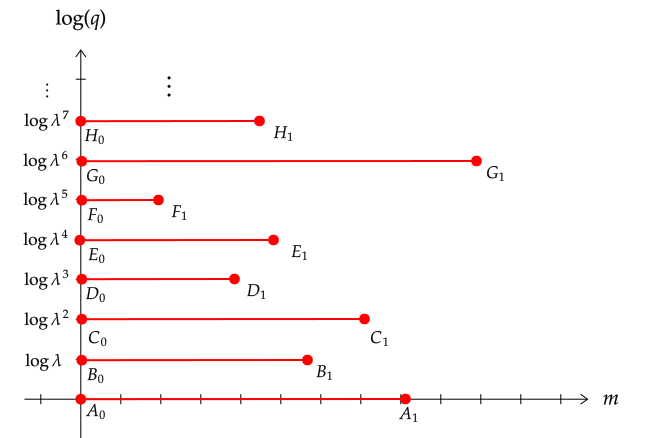
\includegraphics[scale=0.5]{figures/tikz/individual_product_line_dynamics.png}
	

\tikzset{every picture/.style={line width=0.75pt}} %set default line width to 0.75pt        

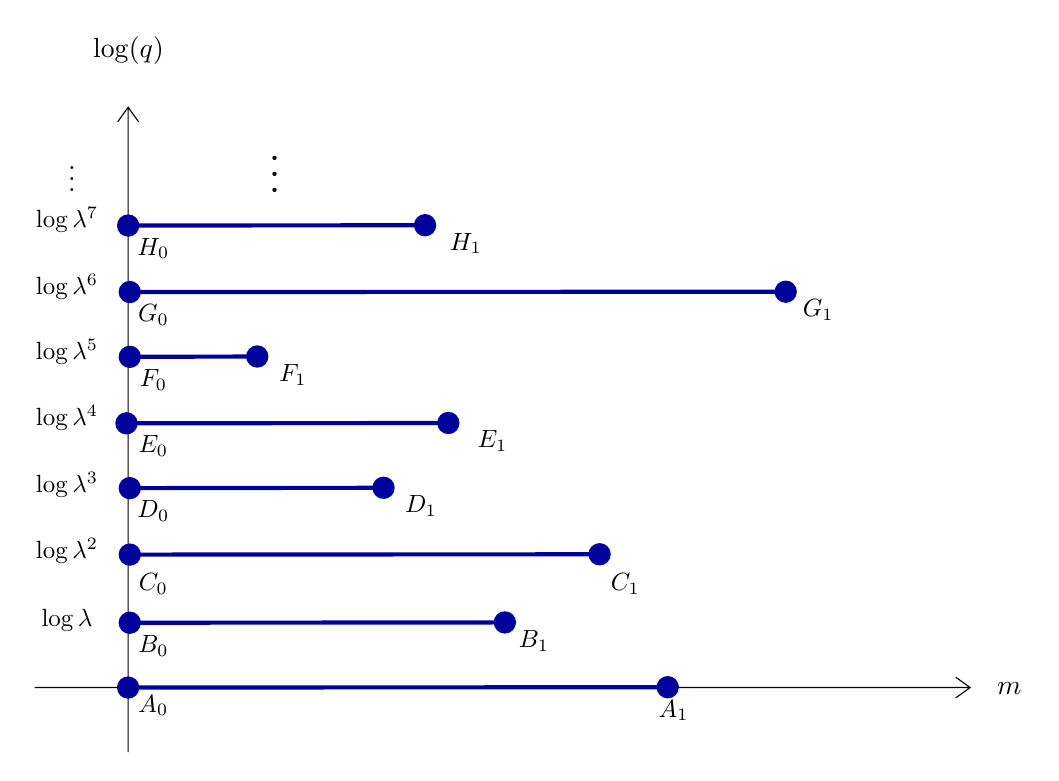
\begin{tikzpicture}[x=0.75pt,y=0.75pt,yscale=-1,xscale=1]
%uncomment if require: \path (0,436); %set diagram left start at 0, and has height of 436

%Shape: Axis 2D [id:dp5962309555056176] 
\draw  (23.9,406.93) -- (474.68,406.93)(68.98,127.34) -- (68.98,438) (467.68,401.93) -- (474.68,406.93) -- (467.68,411.93) (63.98,134.34) -- (68.98,127.34) -- (73.98,134.34)  ;
%Straight Lines [id:da5785444046568369] 
\draw [color={rgb, 255:red, 0; green, 0; blue, 155 }  ,draw opacity=1 ][line width=1.5]    (68.98,406.93) -- (328.96,406.77) ;
\draw [shift={(328.96,406.77)}, rotate = 359.96] [color={rgb, 255:red, 0; green, 0; blue, 155 }  ,draw opacity=1 ][fill={rgb, 255:red, 0; green, 0; blue, 155 }  ,fill opacity=1 ][line width=1.5]      (0, 0) circle [x radius= 4.36, y radius= 4.36]   ;
\draw [shift={(68.98,406.93)}, rotate = 359.96] [color={rgb, 255:red, 0; green, 0; blue, 155 }  ,draw opacity=1 ][fill={rgb, 255:red, 0; green, 0; blue, 155 }  ,fill opacity=1 ][line width=1.5]      (0, 0) circle [x radius= 4.36, y radius= 4.36]   ;
%Straight Lines [id:da8891623197358631] 
\draw [color={rgb, 255:red, 0; green, 0; blue, 155 }  ,draw opacity=1 ][line width=1.5]    (69.78,375.71) -- (250.49,375.55) ;
\draw [shift={(250.49,375.55)}, rotate = 359.95] [color={rgb, 255:red, 0; green, 0; blue, 155 }  ,draw opacity=1 ][fill={rgb, 255:red, 0; green, 0; blue, 155 }  ,fill opacity=1 ][line width=1.5]      (0, 0) circle [x radius= 4.36, y radius= 4.36]   ;
\draw [shift={(69.78,375.71)}, rotate = 359.95] [color={rgb, 255:red, 0; green, 0; blue, 155 }  ,draw opacity=1 ][fill={rgb, 255:red, 0; green, 0; blue, 155 }  ,fill opacity=1 ][line width=1.5]      (0, 0) circle [x radius= 4.36, y radius= 4.36]   ;
%Straight Lines [id:da62109240629908] 
\draw [color={rgb, 255:red, 0; green, 0; blue, 155 }  ,draw opacity=1 ][line width=1.5]    (69.78,342.88) -- (260.1,342.75) -- (296.13,342.72) ;
\draw [shift={(296.13,342.72)}, rotate = 359.96] [color={rgb, 255:red, 0; green, 0; blue, 155 }  ,draw opacity=1 ][fill={rgb, 255:red, 0; green, 0; blue, 155 }  ,fill opacity=1 ][line width=1.5]      (0, 0) circle [x radius= 4.36, y radius= 4.36]   ;
\draw [shift={(69.78,342.88)}, rotate = 359.96] [color={rgb, 255:red, 0; green, 0; blue, 155 }  ,draw opacity=1 ][fill={rgb, 255:red, 0; green, 0; blue, 155 }  ,fill opacity=1 ][line width=1.5]      (0, 0) circle [x radius= 4.36, y radius= 4.36]   ;
%Straight Lines [id:da3991972176156211] 
\draw [color={rgb, 255:red, 0; green, 0; blue, 155 }  ,draw opacity=1 ][line width=1.5]    (68.18,279.63) -- (223.27,279.47) ;
\draw [shift={(223.27,279.47)}, rotate = 359.94] [color={rgb, 255:red, 0; green, 0; blue, 155 }  ,draw opacity=1 ][fill={rgb, 255:red, 0; green, 0; blue, 155 }  ,fill opacity=1 ][line width=1.5]      (0, 0) circle [x radius= 4.36, y radius= 4.36]   ;
\draw [shift={(68.18,279.63)}, rotate = 359.94] [color={rgb, 255:red, 0; green, 0; blue, 155 }  ,draw opacity=1 ][fill={rgb, 255:red, 0; green, 0; blue, 155 }  ,fill opacity=1 ][line width=1.5]      (0, 0) circle [x radius= 4.36, y radius= 4.36]   ;
%Straight Lines [id:da08688218265034209] 
\draw [color={rgb, 255:red, 0; green, 0; blue, 155 }  ,draw opacity=1 ][line width=1.5]    (69.78,310.85) -- (192.04,310.69) ;
\draw [shift={(192.04,310.69)}, rotate = 359.92] [color={rgb, 255:red, 0; green, 0; blue, 155 }  ,draw opacity=1 ][fill={rgb, 255:red, 0; green, 0; blue, 155 }  ,fill opacity=1 ][line width=1.5]      (0, 0) circle [x radius= 4.36, y radius= 4.36]   ;
\draw [shift={(69.78,310.85)}, rotate = 359.92] [color={rgb, 255:red, 0; green, 0; blue, 155 }  ,draw opacity=1 ][fill={rgb, 255:red, 0; green, 0; blue, 155 }  ,fill opacity=1 ][line width=1.5]      (0, 0) circle [x radius= 4.36, y radius= 4.36]   ;
%Straight Lines [id:da027938631411597137] 
\draw [color={rgb, 255:red, 0; green, 0; blue, 155 }  ,draw opacity=1 ][line width=1.5]    (69.78,247.6) -- (131.19,247.44) ;
\draw [shift={(131.19,247.44)}, rotate = 359.85] [color={rgb, 255:red, 0; green, 0; blue, 155 }  ,draw opacity=1 ][fill={rgb, 255:red, 0; green, 0; blue, 155 }  ,fill opacity=1 ][line width=1.5]      (0, 0) circle [x radius= 4.36, y radius= 4.36]   ;
\draw [shift={(69.78,247.6)}, rotate = 359.85] [color={rgb, 255:red, 0; green, 0; blue, 155 }  ,draw opacity=1 ][fill={rgb, 255:red, 0; green, 0; blue, 155 }  ,fill opacity=1 ][line width=1.5]      (0, 0) circle [x radius= 4.36, y radius= 4.36]   ;
%Straight Lines [id:da3281189416601338] 
\draw [color={rgb, 255:red, 0; green, 0; blue, 155 }  ,draw opacity=1 ][line width=1.5]    (69.78,216.38) -- (385.8,216.22) ;
\draw [shift={(385.8,216.22)}, rotate = 359.97] [color={rgb, 255:red, 0; green, 0; blue, 155 }  ,draw opacity=1 ][fill={rgb, 255:red, 0; green, 0; blue, 155 }  ,fill opacity=1 ][line width=1.5]      (0, 0) circle [x radius= 4.36, y radius= 4.36]   ;
\draw [shift={(69.78,216.38)}, rotate = 359.97] [color={rgb, 255:red, 0; green, 0; blue, 155 }  ,draw opacity=1 ][fill={rgb, 255:red, 0; green, 0; blue, 155 }  ,fill opacity=1 ][line width=1.5]      (0, 0) circle [x radius= 4.36, y radius= 4.36]   ;
%Straight Lines [id:da5404789458766659] 
\draw [color={rgb, 255:red, 0; green, 0; blue, 155 }  ,draw opacity=1 ][line width=1.5]    (68.98,184.35) -- (212.06,184.19) ;
\draw [shift={(212.06,184.19)}, rotate = 359.94] [color={rgb, 255:red, 0; green, 0; blue, 155 }  ,draw opacity=1 ][fill={rgb, 255:red, 0; green, 0; blue, 155 }  ,fill opacity=1 ][line width=1.5]      (0, 0) circle [x radius= 4.36, y radius= 4.36]   ;
\draw [shift={(68.98,184.35)}, rotate = 359.94] [color={rgb, 255:red, 0; green, 0; blue, 155 }  ,draw opacity=1 ][fill={rgb, 255:red, 0; green, 0; blue, 155 }  ,fill opacity=1 ][line width=1.5]      (0, 0) circle [x radius= 4.36, y radius= 4.36]   ;

% Text Node
\draw (39.52,374.75) node [scale=0.9]  {$\log \lambda $};
% Text Node
\draw (69.14,100.12) node [scale=1]  {$\log( q)$};
% Text Node
\draw (493.49,407.37) node [scale=1]  {$m$};
% Text Node
\draw (39.52,341.12) node [scale=0.9]  {$\log \lambda ^{2}$};
% Text Node
\draw (39.52,309.09) node [scale=0.9]  {$\log \lambda ^{3}$};
% Text Node
\draw (39.52,277.07) node [scale=0.9]  {$\log \lambda ^{4}$};
% Text Node
\draw (39.52,245.04) node [scale=0.9]  {$\log \lambda ^{5}$};
% Text Node
\draw (39.52,213.81) node [scale=0.9]  {$\log \lambda ^{6}$};
% Text Node
\draw (39.52,181.79) node [scale=0.9]  {$\log \lambda ^{7}$};
% Text Node
\draw (81.15,415.58) node [scale=0.9]  {$A_{0}$};
% Text Node
\draw (331.76,417.98) node [scale=0.9]  {$A_{1}$};
% Text Node
\draw (81.15,386.76) node [scale=0.9]  {$B_{0}$};
% Text Node
\draw (264.5,384.36) node [scale=0.9]  {$B_{1}$};
% Text Node
\draw (81.15,357.13) node [scale=0.9]  {$C_{0}$};
% Text Node
\draw (308.54,357.13) node [scale=0.9]  {$C_{1}$};
% Text Node
\draw (41.92,157.77) node   {$\vdots $};
% Text Node
\draw (81.15,290.68) node [scale=0.9]  {$E_{0}$};
% Text Node
\draw (244.49,288.28) node [scale=0.9]  {$E_{1}$};
% Text Node
\draw (81.15,321.9) node [scale=0.9]  {$D_{0}$};
% Text Node
\draw (210.06,319.5) node [scale=0.9]  {$D_{1}$};
% Text Node
\draw (81.15,258.65) node [scale=0.9]  {$F_{0}$};
% Text Node
\draw (148.41,256.25) node [scale=0.9]  {$F_{1}$};
% Text Node
\draw (81.15,227.42) node [scale=0.9]  {$G_{0}$};
% Text Node
\draw (401.42,225.02) node [scale=0.9]  {$G_{1}$};
% Text Node
\draw (81.15,195.4) node [scale=0.9]  {$H_{0}$};
% Text Node
\draw (231.68,193) node [scale=0.9]  {$H_{1}$};
% Text Node
\draw (139.6,153.76) node [scale=1.44]  {$\vdots $};


\end{tikzpicture}

	\caption{This figure illustrates the dynamics of an individual good $j$ in the equilibrium of the model. All goods $j$ start at point $A_0$. A typical path is given by the red lines, moving left to right to $A_1$ then jumping to $B_0$ before continuing to drift to $B_1$, jump to $C_0$, and so on.}
	\label{individual_product_line_dynamics}
\end{figure}

\subsection{Equilibrium}

As mentioned previously, household risk-neutrality implies $r_t = \rho$ in equilibrium.

\subsubsection{Static optimization}

The model gains significant tractability from the fact that static production decisions are entirely separable from dynamic R\&D decisions. Below I solve the equilibrium fo the static side of the model, given an allocation to R\&D labor $L_{RD}$. 

Final goods producer optimization implies the following inverse demand function for intermediate goods, 
\begin{align*}
p_j &= L_F^{\beta} q_j^{\beta} k_j^{-\beta}	
\end{align*}

\paragraph{Quality gaps and limit pricing} Let $\bar{q}_j(t)$ denote the highest quality level of good $j$ available in the economy at time $t$. As mentioned before, typically there is limit pricing, and the markup charged by the technology leader in line $j$ would depend on his gap relative to the next laggard, e.g. \cite{baslandze_spinout_2019} or \cite{aghion_competition_2005}, only equating to the monopolistic competition markup for large enough gaps. In this model, I abstract from limit pricing (feasible due to the CES specification), using an assumption borrowed from \cite{akcigit_growth_2018}. At each time $t$, intermediate goods firms play a two-stage Bertrand competition game. In the first stage, participants bear a cost of $\varepsilon > 0$ units of the final good in exchange for a right to compete in the product market. In the second stage, they engage in Bertrand competition. Limit pricing in the second stage Bertrand game implies that all producers not on the frontier will earn zero profits; therefore, they do not pay the entry cost. 

In this setup, intermediate goods producers maximize profits according to
\begin{align}
\pi(q_j) = \max_{k_j \ge 0} \Big\{ L_F^{\beta} q_j^{\beta} k_j^{1-\beta} - \frac{\overline{w}}{Q} k_j \Big\} \label{incumbent_profit}
\end{align}

where $\overline{w}$ is the equilibrium final goods / intermediate goods wage.
This yields optimal pricing, labor demand and production of intermediate goods,
\begin{align}
k_j &= \Big[ \frac{(1-\beta) Q}{\overline{w}} \Big]^{1/\beta}L_F q_j  \label{optimal_k}\\
l_j &= k_j / Q \label{optimal_l}\\
p_j &= \frac{\overline{w}}{(1-\beta) Q} \label{optimal_p}
\end{align}

Substituting (\ref{optimal_k}) into the first-order condition for final goods firm optimal labor demand yields a closed form expression for the equilibrium wage $\overline{w}$:
\begin{align}
\overline{w} &= C(\beta) Q \label{wbar} \\
C(\beta) &= \beta^{\beta} (1-\beta)^{1-2\beta} \label{def_cbeta}
\end{align}

Substituting (\ref{optimal_k}) and (\ref{wbar}) into the expression for profit in (\ref{incumbent_profit}) yields
\begin{align}
\pi_j &= (1-\beta) C(\beta) L_F q_j \label{profits_eq}
\end{align}

Substituting (\ref{optimal_k}) into (\ref{optimal_l}) and integrating $L_I = \int_0^1 l_j dj$ yields aggregate labor allocated to intermediate goods production,
\begin{align}
L_I &= \Big( \frac{1-\beta}{C(\beta)} \Big)^{1 / \beta} L_F \label{intermediate_goods_labor}
\end{align}

and substituting (\ref{intermediate_goods_labor}) into the labor resource constraint (\ref{labor_resource_constraint}) yields
\begin{align}
L_F &= \frac{1 - L_{RD}}{1 + \Big(\frac{1-\beta}{C(\beta)}\Big)^{1/\beta}}
\end{align}

The value of $L_{RD}$ is determined endogenously by incumbents' and entrants' innovation decisions, described in the next subsection. Output can be computed by substituting (\ref{optimal_k}) into (\ref{final_goods_production}), 
\begin{align}
Y = \frac{(1-\beta)^{1-2\beta}}{\beta^{1-\beta}} Q L_F \label{flow_output}
\end{align}
\subsubsection{Dynamic optimization}

I will solve for an equilibrium of the model which is a balanced growth path. In such an equilibrium, output, consumption and average quality in the economy grow at a constant and equal exponential rate, innovation rate in line $j$ depends only on $m_j$ and the distribution of $m_j$, $F(m) = \mathrm{Pr}_j\{m_j < m\}$, is constant. 

The join distribution of $(m_j,q_j)$ is non-stationary due to the long-run growth in $Q$; however, one might have expected the joint distribution of $(m_j,\tilde{q}_j)$ to be stationary, where $\tilde{q}_j = q_j/Q$. This appears to present a problem because while the firm problem because certain computations rely on firm-level $\tilde{q}_j$: aggregate R\&D labor demand, aggregate growth and the contribution to the law of motion of $m_j$ from non-WSO spinouts. It turns out that because all of these effects are \textit{linear}, all that is required for balanced growth is that $\Gamma(m) = \mathbb{E}\Big[ \tilde{q} \Big| m \Big]$ be constant on the BGP (given that innovation decisions and outcomes depend solely on $m$). In the section below (\textbf{link}) I show that this is indeed the case. Intuitively, while the distribution of $\tilde{q}$ fans out over time due to random shocks and no low exit threshold, its conditional means remain stationary. 

Next, note that the state variable of a good $j$ is $(q_j,m_j,t)$, where $t$ allows dependence on time-varying rates of creative destruction (not the case on the BGP) or economy-wide average quality $Q = \int_{q,m} q  \cdot d\mu(q,m,t)$. Similarly, let $W(q,m,t)$ denote value per spinout idea: that is, a mass $m_{ij}$ of ideas for a good $j$ is worth $m_{ij} W(q_j,m_j,t)$.

\paragraph{Households}

Individuals are risk neutral and can borrow and lend instantaneous risk-free bonds while satisfying a no Ponzi-game condition. This implies that their objective is to maximize the present discounted value of their wages and profits from founding firms (\textbf{theorem?}). Because founding and owning a firm does not require labor, entrepreneurship decisions are completely separate from labor supply decisions. Labor supply is allocated in order to maximize the value of the labor endowment. Denote this value by $U_{labor}$. 

The equilibrium wage paid to R\&D workers not bound by non-competes will depend on the individual state of the product, as this affects the value of the spinouts ideas generated by the R\&D worker. Let $w^{NCA}(q,m,t),w(q,m,t)$ denote the equilibrium wages required by R\&D employees bound (not bound) by an NCA.

Given this, $U_{labor}$ satisfies the HJB equation
\begin{align}
\rho U_{labor} &= \max_{l_{q,m}(\cdot),l_I,l_F} \bar{w}(t) (l_I + l_F) \nonumber\\
&+ \int_{q,m} l_{RD} (q,m) \Bigg(x(q,m,t) \hat{w}^{NCA}(q,m,t) + \Big(1-x(q,m,t) \Big)\hat{w}(q,m,t))  \Bigg) d\mu(q,m,t) \nonumber  \\
\textrm{subject to: }  & l_{RD}(\cdot) \ge 0, l_I \ge 0, l_F \ge 0  \nonumber \\
& l_I + l_F + \int_{q,m} l_{RD}(q,m) d\mu(q,m,t) \le 1 
\end{align}

where $x(q,m,t)$ is equal to 1 if and only if product lines in state $(q,m,t)$ impose an NCA, $l_{RD}(q,m)$ is the average labor supplied by the individual to products in state $(q,m)$,  $\bar{w}(t)$ is the production wage and $\hat{w}^{NCA}(q,m,t),\hat{w}(q,m,t)$ are the effective R\&D wages from the perspective of the employee bound / not-bound by a non-compete, respectively, taking into account the profits from future spinouts: 
\begin{align}
\hat{w}(q,m,t) &=  w(q,m,t) + \nu \Big( \overbrace{\theta \frac{Q_t}{q} W(q,m,t)}^{\textrm{WSOs}} + \overbrace{(1-\theta) \mathcal{W}(t)}^{\textrm{Non-WSOs}} \Big) \label{worker_effective_wage}\\
\hat{w}^{NCA}(q,m,t) &= w^{NCA}(q,m,t) + \nu \underbrace{(1-\theta) \mathcal{W}(t)}_{\textrm{Only Non-WSOs}} \label{worker_effective_wage_NCA}\\ 
\mathcal{W}(t) &= \int_{q,m} W(q,m,t) d\mu(q,m,t)
\end{align}

In equilibrium, the worker is indifferent between all forms of employment. This means that whenever
$x(q,m,t) = 0$, 
\begin{align}
\hat{w}(q,m,t) &= \bar{w}(t) \label{wage_rd}
\end{align}

And whenever $x(q,m,t) = 1$, 
\begin{align}
\hat{w}^{NCA}(q,m,t) &= \bar{w}(t) \label{wage_rd_NCA}
\end{align}



\paragraph{Incumbents}

Let $\pi(q,m,t) = \pi q$ denote flow profits from sales of the intermediate good and let $\tau(q,m,t) = \tau_E(q,m,t) + \tau_S(q,m,t)$ denote the arrival rate of creative destruction by entrants and spinouts. Let $\bar{\sigma}$ denote the equilibrium flow increase in $m$ due to non-WSO spinouts. 

The incumbent value function satisfies the HJB equation
\begin{align}
\big(\rho + \tau^E(q,m,t)& \big)V(q,m,t) = \pi q + \bar{\sigma} V_m + V_t  \nonumber \\
&+ \max_{x \in \{0,1\}, z \ge 0} \Bigg\{ z \Big( z^{-\psi} \chi \big( V(\lambda q, 0, t) - V(q,m,t) \big)  \nonumber \\
&- \frac{q}{Q_t} x w^{NCA}(q,m,t) - (1-x) \big( \frac{q}{Q_t} w(q,m,t) - \theta \nu V_m \big)\Big)    \Bigg\} \label{HJB_I}
\end{align}

Define the incumbent's effective cost of R\&D without and with an NCA, 
\begin{align}
\tilde{w}(q,m,t) &= \frac{q}{Q_t} w(q,m,t) - \theta \nu V_m(q,m,t)  \label{incumbent_effective_wage} \\
\tilde{w}^{NCA}(q,m,t) &= \frac{q}{Q_t} w^{NCA}(q,m,t)  \label{incumbent_effective_wage_NCA} 
\end{align}

That is, the effective cost of R\&D is the wage plus the reduction in firm value from the resulting marginal increase in the stock of spinouts attempting entry, $m$. This is because higher $m$ implies a higher hazard rate of losing the monopoly position. It follows from the HJB that the incumbent uses a non-compete (chooses $x = 1$) whenever it means his effective cost of R\&D is lower: $\tilde{w} > \tilde{w}^{NCA}$. 

A higher wage is required to attract labor when a non-compete is imposed, since it eliminates the expected value of the employee's future WSOs. The gap in wages required to attract labor is equal to the expected discounted present value of WSO formation to the worker. Using (\ref{worker_effective_wage}), (\ref{worker_effective_wage_NCA}), (\ref{wage_rd}), (\ref{wage_rd_NCA}), (\ref{incumbent_effective_wage}), and (\ref{incumbent_effective_wage_NCA}), it follows that (suppressing function arguments)
\begin{align}
\tilde{w}^{NCA} &= \tilde{w} + \overbrace{\nu \theta }^{\textrm{WSO formation}} \Bigg( \underbrace{\theta \nu V_m}_{\textrm{Harm to incumbent}} + \overbrace{\nu \theta W}^{\textrm{Value to employee}} \Bigg)
\end{align} 

That is, the incumbent uses a non-compete whenever the ex-ante bilateral value of knowledge spillovers from the incumbent to the R\&D employee is positive. Even absent explicit bargaining, equilibrium ensures the use of the bilaterally optimal contract (given the available contract space). Negative social consequences of non-competes in this model therefore must arise from externalities and general equilibrium effects rather than direct harm to those bound by them.\footnote{This is also the case in the models developed in \cite{baslandze_spinout_2019} and \cite{shi_restrictions_2018}. In fact, there is some empirical evidence that non-compete contracts can be damaging to workers themselves. For example, in some cases a non-compete can be used as a way to extract more rent from the worker after a job has already been accepted. See the discussion in \cite{starr_consider_2018}.} This is summarized by the optimal non-compete policy
\begin{align}
	x^*(q,m,t) &= \begin{cases}
	0 & \textrm{if } \tilde{w}^{NCA}(q,m,t) \ge \tilde{w}(q,m,t) \\
	1 & \textrm{otherwise} 
	\end{cases}
\end{align}

Optimal R\&D by incumbents is determined by the first-order condition
\begin{align}
z^*(q,m,t) &= \Bigg( \frac{x^*(q,m,t) \tilde{w}^{NCA}(q,m,t) + (1-x^*(q,m,t))\tilde{w}(q,m,t)}{\chi(1-\psi) \Big(V(\lambda q, 0, t) - V(q,m,t) \Big)}\Bigg)^{-1/\psi}
\end{align}

leading to an arrival rate
\begin{align}
	\tau^*(q,m,t) &= \chi z^*(q,m,t)^{1-\psi} 
\end{align}

\paragraph{Spinout ideas}

The value of a spinout idea $W(q,m,t)$ satisfies the HJB
\begin{align}
(\rho  + \tau_E + \tau_S& + \tau_I)W(q,m,t) = W_t(q,m,t) + \bar{\sigma}W_m(q,m,t) \nonumber \\
+& \max_{0 \le z \le 1} \Big\{ \underbrace{\chi_S z (z_E + z_S)^{-\hat{\psi}} (1-\kappa) V(\lambda q,0,t)}_{\textrm{Flow value of potential innovation}} - \underbrace{\Big(\frac{q}{Q_t}\Big) z w(q,m,t)}_{\textrm{R\&D cost}} \Big\} \label{HJB_S}
\end{align}

There are three important differences relative to the incumbent's problem. First, because each spinout is infinitesimal, individual spinouts in line $j$ have no effect on the overall creative destruction rate in line $j$. Second, because employment at spinouts does not generate further spinout ideas for employees, spinouts pay the production wage for R\&D employees. As mentioned before, this can be relaxed, but I have no data on R\&D by spinouts with which to discipline the necessary parameters.\footnote{If this were relaxed, because spinouts are infinitesimal, their effective wage paid would equal the nominal wage, because they have no individual effect on the dynamics of the state variable $m_j$.} Finally a cost $\kappa V(\lambda q, 0, t)$ in terms of the final good must be paid upon entry, reducing the expected payoff from a successful innovation. 

\paragraph{Equilibrium entry behavior}

Free entry by ordinary entrants imposes the following condition on $z_E(q,m,t)$, 
\begin{align}
\chi_E \big( z_E(q,m,t) + z_S(q,m,t) \big)^{-\hat{\psi}} \Big(\frac{q}{Q_t}\Big)^{-1}  (1-\kappa) V(\lambda q,0,t)  &= \bar{w}(t)\label{free_entry_entrants}
\end{align}
with equality if $z_E(q,m,t) > 0$. 

Provided that $\chi_S > \chi_E$, spinouts price ordinary entrants out of the innovation race as $m$ increases. During this process, free entry of ordinary entrants implies that $z_S(q,m,t) + z_E(q,m,t)$ remains constant. Once $z_E(q,m,t) = 0$, spinouts continue to enter until $m$ reaches the free entry mass $M(q,t) > 0$ defined by
\begin{align}
\chi_S  M(q,t)^{-\hat{\psi}}\Big(\frac{q}{Q_t}\Big)^{-1} (1-\kappa) V(\lambda q,0,t)  &= \overline{w}(t) \label{free_entry_spinouts}
\end{align}

That is, for $m \ge M(q,t)$ have $z_S(q,m,t) = M(q,t)$ and for $m < M(q,t)$ have $z_S(m,q,t) = m$. It also follows that $W(q,M(q,t),t) = 0$, which can be used as a terminal condition for solving (\ref{HJB_S}).


\subsubsection{Linear scaling in $q$}

I guess and verify that $V(q,m,t) = q V(m)$ and $W(q,m,t) = qW(m)$ for some functions $V(m)$ and $W(m)$ (abusing notation slightly). Similarly, I conjecture that $x,z_I,z_E,zS,\tau_E,\tau_S$ are functions of $m$ exclusively, that $M(q,t) \equiv M^*$, and that $L_F,L_I,L_{RD}$ are constant, which by (\ref{profits_eq}) implies that $\pi(q,m,t) = \pi q$. Then (\ref{wbar}) implies $\bar{w}(t) = Q_t \bar{w}$ and (\ref{wage_rd}), (\ref{wage_rd_NCA}), (\ref{incumbent_effective_wage}), and (\ref{incumbent_effective_wage_NCA}) imply that $w(q,m,t) = Q_t w(m),w^{NCA}(q,m,t) = Q_tw^{NCA}(m)$, $\hat{w}(q,m,t) = Q_t \hat{w}(m)$, $\hat{w}^{NCA}(q,m,t) = Q_t \hat{w}^{NCA}(m)$, $\tilde{w}(q,m,t) = q \tilde{w}(m)$ and $\tilde{w}^{NCA}(q,m,t) = q\tilde{w}^{NCA}(m)$.

To verify the guess is consistent with firm and individual dynamic optimization, substitute into (\ref{HJB_I}) and eliminate the common factor $q$, yielding
\begin{align}
(r + \tau_E(m) + &\tau_S(m)) V(m) = \pi + \bar{\sigma}V'(m) \nonumber \\
&+ \max_{z \ge 0, x \in \{0,1\}} \Big\{  \chi z \phi_I(z) \Big[\lambda V(0) - V(m) \Big] - z \Big(x \tilde{w}^{NCA}(m) + (1-x) \tilde{w}(m) \Big) \Big\} \label{BGP_HJB_I}
\end{align} 

Similary, substitute into (\ref{HJB_S}) to obtain
\begin{align}
(r + \tau_E(m) + &\tau_S(m) + \tau_I(m))W(m) = \sigma(m) W'(m) \nonumber \\
&+ \max_{0 \le z \le \xi} \Big\{  \chi_S z (z_E(m) + z_S(m))^{-\hat{\psi}} (1-\kappa) \lambda V(0) - z \bar{w} \Big\} \label{BGP_HJB_S} 
\end{align}

where
\begin{align}
\sigma(m) &= \nu \theta z_I(m) + \bar{\sigma} 
\end{align}

Given these HJBs, optimal policies are confirmed as functions of only $m$ as well, which confirms the BGP guess:
\begin{align}
x^*(m) &= \textbf{1}_{\tilde{w}(m) > \tilde{w}^{NCA}(m)} \big(m\big) \\
z_I^*(m) &= \Bigg( \frac{x^*(m) \tilde{w}^{NCA}(m) + (1-x^*(m)) \tilde{w}(m)}{\chi (1-\psi) \Big(\lambda V(0) - V(m) \Big)} \Bigg)^{-1/\psi} \\
z_E^*(m) &= \max \Bigg\{0, \Big(\frac{\overline{w}}{\chi_E (1-\kappa) \lambda V(0)} \Big)^{-1 / \hat{\psi}} - z_S^*(m)\Bigg\} \\
z_S^*(m) &= \min(m,M^*) \\
M^* &= \Big(\frac{\overline{w}}{\chi_S (1-\kappa) \lambda V(0)} \Big)^{-1 / \hat{\psi}}
\end{align}


\paragraph{Aggregate distributions} 

On the balanced growth path, $Q_t = \int_{q,m} d\mu(q,m,t)$ grows at a constant rate $g$. Given the guess that innovations occur on a good $j$ as a function only of $m$, I show below that there exists stationary distribution in $m$-space, with density $\mu(m)$, together with a function $\Gamma(m) = \mathbb{E}_t[q/Q_t|m]$. The density $\mu(m)$ satisfies Kolmogorov Forward Equation
\begin{align}
0 = - \frac{d}{dm} \Big( \sigma(m) \mu(m) \Big) - \tau(m) \mu(m)  \label{KF_equation}
\end{align}
where
\begin{align}
\tau(m) &= \tau_I(m) + \tau_S(m) + \tau_E(m) 
\end{align}

This ODE has solutions of the form
\begin{align}
\mu(m) &= C_\mu e^{-\int_0^m \frac{\sigma'(m') + \tau(m')}{\sigma(m')}} dm' \label{KF_solution_1}
\end{align}

Because $\mu(m)$ is a probability density function, $C_\mu$ is determined by
\begin{align}
1 = \int_0^{\infty} \mu(m) dm \label{KF_solution_2}
\end{align}

To compute $\Gamma(m)$, define $s(m)$ as the equilibrium (deterministic) amount of time to reach state $m$ from state $0$ conditional on there being no innovations, 
\begin{align}
s(m) &= \int_0^m \frac{1}{\sigma(m')} dm'
\end{align}

Define $\tilde{\Gamma}(s') = \Gamma(s^{-1}(s'))$. Absent any innovation, $q/Q_t$ decreases at rate $g$. Therefore, $\tilde{\Gamma}(s)$ decays at rate $g$, $\tilde{\Gamma}(s) = C_{\Gamma} e^{-gs}$. Recover $\Gamma(m)$ using $\Gamma(m) = \tilde{\Gamma}(s(m))$. Finally, $C_{\Gamma}$ is determined by the law of iterated expectations,\footnote{It is possible to also derive the condition $C_{\Gamma} = \lambda \int_0^{\infty} \Gamma(m) \tau(m) \mu(m) dm$. This equation can be shown to be redundant (\textbf{appendix})}
\begin{align}
\int_0^{\infty} \Gamma(m) \mu(m) dm = 1
\end{align}

\paragraph{Aggregate growth, R\&D labor demand, and non-WSO spinouts}

Given aggregate distributions $\mu(m),\Gamma(m)$ and product-level innovation rates $\tau(m) = \tau_I(m) + \tau_S(m) + \tau_E(m)$, the growth rate of TFP is given by
\begin{align}
g &= (\lambda -1) \int_0^{\infty} \tau(m) \Gamma(m) \mu(m) dm 
\end{align}

The growth equation aggregates across products in $m$-space using the stationary density $\mu(m)$. For each $m$, the contribution to growth is the product of the rate of innovation $\tau(m)$, the average relative quality $\Gamma(m)$, and $(\lambda -1)$, the proportional improvement in quality per innovation.

R\&D labor demand is given by 
\begin{align*}
L_{RD} &= \int_0^{\infty} \big (z_I(m) + z_S(m) + z_E(m)\big)\Gamma(m)\mu(m) dm
\end{align*}

Finally, the law of motion of the mass of spinouts for a line with current mass $m$ can be computed as
\begin{align*}
	\dot{m} &= \nu \Big( \theta z^I(m) + (1-\theta) \int_0^{\infty} z^I(m') \Gamma(m') \mu(m') dm' \Big)
\end{align*}


\subsubsection{Solution algorithm}\label{solution_algorithm}

The HJBs given above cannot be solved in closed form. I solve them using a variant of the numerical method described in using method in \cite{achdou_income_2017}. I can then solve the model numerically using the following algorithm.

\begin{enumerate}
	\item Guess $\{g, L_{RD}, w(m), w^{NC}, M, \bar{\sigma} \}$
	\begin{enumerate}
		\item Static equilibrium conditions $\Rightarrow L_I,L_F,\pi$
		\begin{enumerate}
			\item Free entry, etc. $\Rightarrow z_S(m), z_E(m)$
			\item Incumbent HJB $\Rightarrow  V(m),z_I(m)$ 
			\item Update $M$ and check for convergence
		\end{enumerate}
		\item Spinout HJB $\Rightarrow$ $W(m)$
		\item Aggregation $\Rightarrow$ $\mu(m),\gamma(m),g,L_{RD},\bar{\sigma},\mathcal{W}$
		\item Worker indifference $\Rightarrow$ $w(m),w^{NC}$
		\item Check convergence of of $\{g, L_{RD}, w(m), w^{NC}, M, \bar{\sigma} \}$
	\end{enumerate}
\end{enumerate}


\subsection{Efficiency}

The social planner problem now involves controlling the infinite dimensional aggregate state variable $\mu(\cdot), \gamma(\cdot)$ as well as infinite dimensional individual policy functions $z_S(\cdot),z_E(\cdot),z_I(\cdot)$ to maximize welfare, given market clearing and the steady state KF and $\gamma$ equations. I plan to adapt the methods in \cite{nuno_social_2018} to compute the social planner's allocation numerically. Given risk-neutrality, expected utility for a household born in this economy is equal to the expected discounted present value of consumption in the economy at time $t = 0$ with $Q_0 = 1$. 

\section{Calibration and model validation}

\subsection{Calibration}

I calibrate the model using direct and indirect inference, as well as some parameters from the literature when identification using the model is difficult (e.g., R\&D elasticities). 

Table \ref{identification} displays the various parameters to be identified alongside their sources of identification. 

\begin{table}
	\small
	\centering
	\begin{tabular}{rll}
		\toprule \toprule 
		Parameter &  Description & Source / Target\\
		\midrule
		\textbf{Chosen from literature}& \\
		$\psi, \hat{\psi}$ & Curvature of incumbent, entrant R\&D & R\&D regressions from \\
		& technology & literature\\
		& & \\
		\textbf{Matched exactly}&  \\
		$\rho$ & Discount factor & Interest rate \\
		$\beta$ & $\beta^{-1}$ EoS between intermediate goods & Profit / GDP \\
		$\chi_S / \chi_E$ & Spinouts / entrants R\&D prod. & Spinout / entrant hazard \\
		& & of successful exit \\
		$\theta$ & Fraction of spinouts that & WSO reg. coef. divided \\
		& are WSOs & by All Spinout reg. coef. \\
		& \\
		\textbf{Indirect inference}& \\
		$\lambda$ & Step size of innovations & Growth rate \\
		$\chi_I$ & Incumbent R\&D prod. & Fraction of innovations \\
		& &  by incumbent firms \\
		$\kappa$ & Entry cost & R\&D / GDP ratio\\
		$\chi_E$ & Entrant R\&D prod. & Entry rate \\
		$\nu$ & Spinout idea generation rate & Spinout entry rate implied \\
		& & by regressions \\
		\bottomrule
	\end{tabular}
	\captionof{table}{Identification of model parameters.}\label{identification}
\end{table}

\paragraph{Identification of discount rate and intermediate goods elasticity}

The parameter $\rho$ is equal to the interest rate in the equilibrium of the economy. While the model exhibits no risk premium due to risk neutrality, I calibrate $\rho = 0.05$ so that it matches a real interest rate of 5\%, to better reflect the fact that such investments would carry a risk premium in the actual economy. 

The parameter $\beta$ controls both the elasticity of substitution between intermediate goods and the share of income that accrues to final goods labor. I calibrate it by targeting the ratio of profits to GDP, which is about 6\%.\footnote{I believe this is preferrable to calibrating to the R\&D / sales ratio, as in \cite{akcigit_growth_2018}, for two reasons: the R\&D / sales ratio is contaminated by the degree of vertical integration in the supply chain, which is not present in the model, which assumes that intermediate goods firms produce using no intermediate goods of their own.} Using (\ref{profits_eq}) and (\ref{flow_output}) one can show that the profit to final goods output ratio is $\frac{(1-\beta) C(\beta) \beta^{1-\beta}}{(1-\beta)^{1-2\beta}}$, yielding a $\beta = .065$. According to (\ref{optimal_p}), this implies an equilibrium markup of $6.9\%$.

\paragraph{Identification of R\&D curvature parameters}

The parameters $\psi, \hat{\psi}$ govern the curvature of the innovation production function. I choose $\psi = 0.5$, based on microeconometric estimates of (1) the elasticity of patents to R\&D expenditures (citations), and (2) the impact of R\&D tax credits on R\&D expenditures. See the discussion in \cite{akcigit_growth_2018}. 

As discussed previously, $\hat{\psi} > \psi$ in order to capture the fact that entering firms do not coordinate their innovations and therefore run the risk of duplicating projects. A higher value of the parameter $\hat{\psi}$ implies a lower sensitivity of entry to changes in firm value. Absent data with which to discipline, I set a baseline of $\hat{\psi} = 0.7$ and conduct robustness checks where I vary the value of this parameter (\textbf{what values?}).

\paragraph{Identification of R\&D productivity parameters}

The parameters $\lambda, \chi_I, \chi_S, \chi_E, \kappa$ control the productivity of the innovation and entry technology of incumbents and entrants. These parameters jointly affect all moments relating to innovation, so it is not possible to say precisely which moment is identifying the parameter. However, I will give a rough description of where the main discipline is coming from. It is useful to decompose them as follow: $\lambda , \chi_E, \chi_S / \chi_E, \chi_I / \chi_E, \kappa$. 

The aggregate growth rate is of course an important source of identification, as it is increasing in $\lambda$, decreasing in $\kappa$ and increasing in $\chi_E$ holding all other parameters constant. 

Next, the fraction of innovations that are due to new firms -- which I calculate from the NBER USPTO data, using patents as a proxy for number of innovations -- is decreasing in $\chi_I / \chi_E$. However, identification is complicated by the fact that it is also decreasing in $\lambda$: a higher $\lambda$ reduces the gap in innovation incentives for incumbents relative to entrants by reducing the ``business-stealing'' effect, which amplifies the perceived innovation reward by (roughly) a factor $\frac{\lambda}{\lambda-1}$ for entrants relative to incumbents. Given a growth rate $g$, one can match a high fraction of new firm innovations by changing $\chi_I / \chi_E$, or alternatively by lowering $\lambda$ (to increase $\tau_I / \tau_E$) and raising $\chi_E$ to preserve the aggregate growth rate.  

One solution to separate $\lambda$ from $\chi_I / \chi_E$ is to study the frequency with which products are innovated on. Given an entry rate for ordinary entrants (controlled by $\chi_E$) and the fraction innovations undertaken by entrants (controlled by $\chi_I / \chi_E$), the aggregate growth rate pins down $\lambda$. I compute the firm entry rate from the patent data, considering a new firm to be one with no prior history of patenting. In each year, I divide the number of new firms by the total number of patenting firms active that year. I then average across years in my sample period. Note that the relevant entry rate in the model is the rate of successful innovations by entrant firms.

The ratio $\chi_S / \chi_E$ I determine by matching the statistics on the difference in valuation and employment between spinouts and ordinary entrants in my sample. Because ordinary entrants in the model have individually constant returns to scale, and because spinouts have no intensive margin of R\&D spending, there is no notion of the size or valuation of an entrant against which the typical size of a spinout in the model can be compared. I calibrate $\chi_S / \chi_E$ to this relative difference directly.\footnote{With individual returns of elasticity $\alpha \in (0,1)$, the ratio of productivities is the ratio of firm sizes raised to the exponent $(1-\alpha)^{-1} \in (0,1)$. That is, my current framework overestimates the difference in productivity.} Note also that, because $\chi_S / \chi_E$ pertains to the difference in likelihood of successful innovation, I interpret the startups in my data, prior to a successful exit, as not having successfully innovated yet. This is not completely consistent with my interpretation of new patenting firms as entrants, since many startups pre IPO indeed have patents, but it is the closest approximation I currently have.\footnote{One possible modification to harmonize my various interpretations of firm entry is to assume that patenting firms enter only when they file for their first high quality patent, where quality is measured by future citations to the patent. Whether a firm is able to sucessfully exit and / or grow into a firm with high levels of output is likely related to the quality of its patents, although I cannot verify this directly (without significant work) because startups in my data are not linked to the patent data.}

Next, there is a challenge around separately identifying $\kappa$ from $\chi_E$. The issue is that a higher $\kappa$ reduces the overall entry rate. One possibility is to use the fact that an increase in $\kappa$ tends to increase the fraction of entry due to spinouts, since ordinary entrants are usually the marginal firms. However, the parameter $\nu$, which controls the rate at which R\&D produces new spinout ideas, also must be identified off of this moment (see the next subsection), so another moment is needed. A second candidate is based on the observation that $\kappa$ affects the incentives for ordinary entrant, rather than their technology. The natural way to disentangle this from a technological parameter is to use data on the productivity of R\&D. Given the amount of growth in the economy, R\&D productivity is measured by the inputs dedicated to R\&D. Hence, I separate $\kappa$ from the remaining parameters by attempting to match the level of R\&D spending as a fraction of GDP. 

\paragraph{Identification of spinout entry parameters}

The remaining parameters to be calibrated are $\nu$ and $\theta$, which determine the generation of spinout ideas (with $\theta$ controlling the fraction which are in the same industry as the parent). Consider the parameter $\nu$, which controls the rate at which incumbent R\&D spending generates ideas for spinouts. Because each spinout is infinitesimal, $\nu$ does not generate any predictions regarding the number of founders per R\&D dollar or the number of firms per R\&D dollar. This poses a challenge because this is exactly what I measure in the empirical section. 

The model does generate predictions regarding the rate at which R\&D spending and employment by spinouts overall increases as an incumbent performs R\&D. However, I do not have data on R\&D spending by spinout firms. Data on spinout employment is available, but to correspond to the model, it would need to be specifically R\&D employment, and it would need to be compared to a measure of R\&D employment per dollar at the incumbent firm. 

To sidestep these complications, I take an indirect approach to calibrating $\nu$ and $\theta$. First, using the estimated causal relationship between R\&D and total spinout and WSO formation, I compute the fraction of founders in each year which can be attributed to parent firm R\&D and divide these into WSO and non-WSOs. Then, using the estimated difference in the hazard rate of a successful exit for ordinary entrants, WSOs and non-WSO spinouts, I compute the fraction of successful exits that are WSO and non-WSO spinouts caused by parent firm R\&D. As before, I identify successful exit in the data with successful innovation in the model. I can then identify $\nu$ and $\theta$ from the measured successful exit rates due to parent firm R\&D. 

Notice that $\theta$ captures the combination of the relative frequency of WSO ideas and their relative productivity. In order for the model to allow for different productivities of WSO and non-WSO ideas, I would need to add another state variable, since the mass of each type of idea would be relevant to the firm. In addition, the incumbent only cares about the aggregate of these two quantities, since what is relevant is the rate at which R\&D increases the probability of being overtaken by former employees. This does affect spinout decisions, but I strongly conjecture that in an augmented model both forms of spinouts would almost always be above the entry margin, and therefore whether WSOs are modeled as more productive or simply occuring more frequently does not affect their decisions in the equilibrum or alter comparative statics. \textbf{Does this sound right?}

Table \ref{calibration_targets} displays the calibrations targets in the data and in the model. The model matches the targeted moments well. This is not strong validation of the model since there are as many parameters as targeted moments, but it is a start. 


\begin{table}
	\centering
	\captionof{table}{Calibration targets}\label{calibration_targets}
	\begin{tabular}{rll}
		\toprule \toprule
		  & Target & Model \tabularnewline
		\midrule
		\multicolumn{1}{l}{\textbf{Exactly matched}} & &  \tabularnewline
		Interest rate & 5\% & 5\% \tabularnewline
		Profit (\% GDP) & 6\% & 6\% \tabularnewline
		Spinouts / ordinary entrants & 1.3 & 1.3 \tabularnewline
		innovation probability \tabularnewline
		\tabularnewline
		\multicolumn{1}{l}{\textbf{Indirect inference}} & & 
		\tabularnewline
		Growth rate & 1.5\% & 1.35\% 
		\tabularnewline
		R\&D spending (\% GDP) & 1.5\% & 0.9\% 
		\tabularnewline		
		Incumbent innovation share & 0.75 & 0.63
		\tabularnewline
		Entry rate & 0.09 & 0.097
		\tabularnewline
		Spinout entry rate & 0.03 & 0.03
		\tabularnewline
		\bottomrule
	\end{tabular}
\end{table}

Table \ref{calibration_parameters} displays the parameter settings in the calibration above. 

\begin{table}
	\centering
	\captionof{table}{Calibration parameters}\label{calibration_parameters}
	\begin{tabular}{rlll}
		\toprule \toprule
		Parameter & Value & Description \tabularnewline
		\midrule
		$\rho$ & 0.05 & Discount rate \tabularnewline
		$\beta$ & 0.065 & $(1-\beta)^{-1}$ markup\tabularnewline
		$\psi$ & 0.5 & Incumbent R\&D elasticity \tabularnewline
		$\hat{\psi}$ & 0.7 & Entrant R\&D elasticity \tabularnewline
		$\lambda$ & 1.053 & Quality ladder step size \tabularnewline
		$\chi_I$ & 1.43 & Incumbent R\&D productivity \tabularnewline
		$\chi_E$ & 0.22 & Ordinary entrant R\&D productivity \tabularnewline
		$\chi_S$ & 0.29 & Spinout R\&D productivity \tabularnewline
		$\kappa$ & 0.82 & Entry cost \tabularnewline
		$\nu$ & 0.34 & Spinout generation rate \tabularnewline
		$\theta$ & 0.5 & Fraction WSOs\tabularnewline
		\bottomrule
	\end{tabular}
\end{table}



\subsection{Calibrated equilibrium}

In this section I document the properties of the equilibrium that results from the calibration in the previous section. First, \autoref{figure:calibration_HJB_solutions_plot} shows the value functions and R\&D policies of incumbents and spinouts, as a function of $m$. Both value functions are decreasing in $m$ until $M^*$ after which they are constant. This is because, provided $m \le M^*$, higher $m$ increases the hazard rate of creative destruction, reducing the expected duration of the incumbent's monopoly. For $m > M^*$, additional spinout ideas formed do not find it profitable to enter and the hazard rate no longer increases. 

By contrast, both policy functions are increasing in $m$ until $M^*$ and subsequently constant. The spinout policy function is mechanical as spinouts have no intensive margin and as $m$ increases there is a larger mass of spinouts which can choose to enter. The incumbent policy function increases in $m$ due to the ``escape competition'' effect, whereby it pays to innovate when successfully doing so creates more distance from one's competition (i.e., decreases the subsequent hazard rate of creative destruction). That is the case here, since a successfull innovation returns $m$ to zero, reducing the mass of spinouts attempting entry. 

\begin{figure}[]
	\centering
	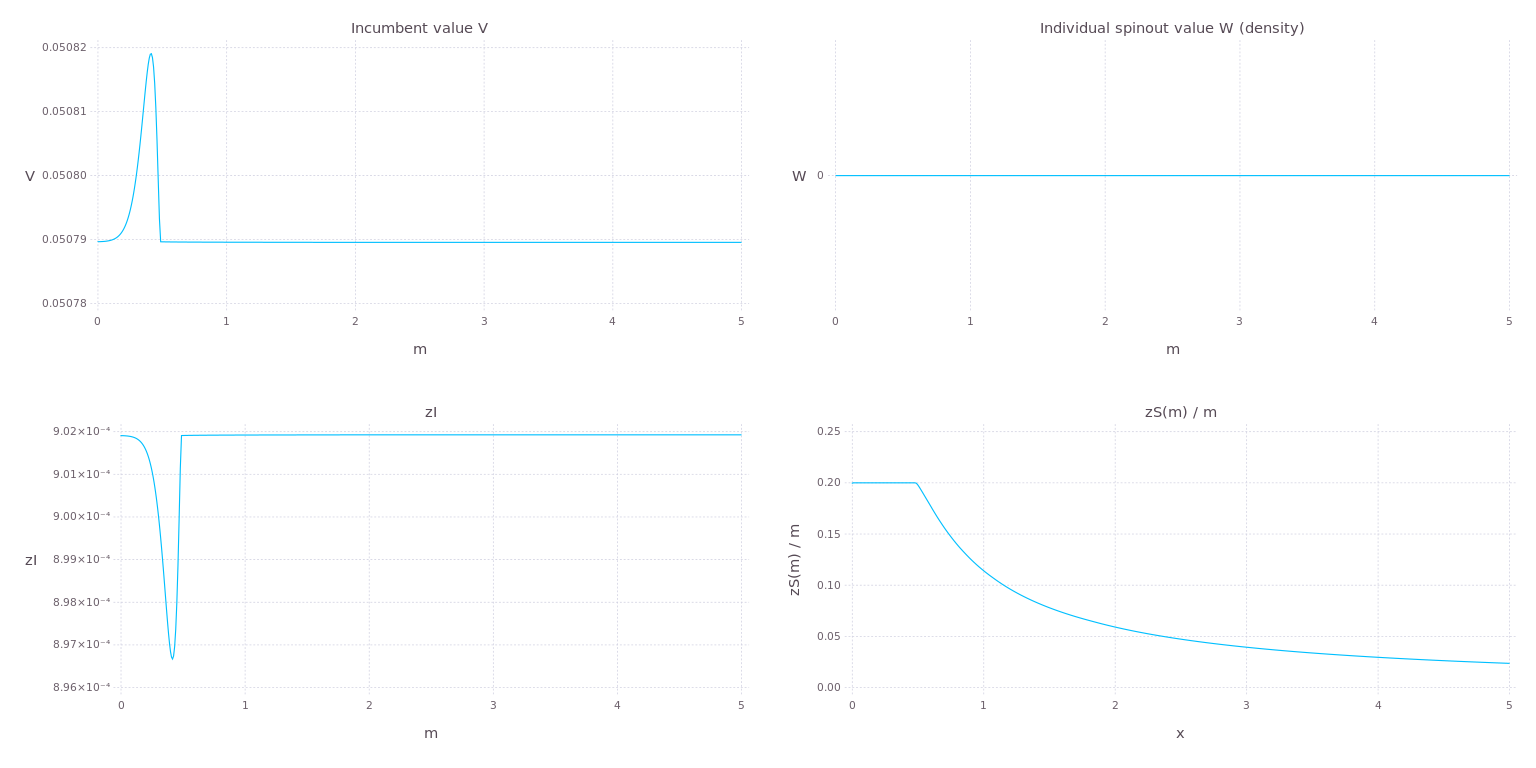
\includegraphics[scale=0.77]{../code/julia/figures/plotsGR/HJB_solutions_plot.pdf}
	\caption{Equilibrium incumbent and spinout value functions and R\&D policy. The upper left panel shows the value function of an incumbent as a decreasing function of the mass $m$ of spinout attempting innovation on his good own good $j$. The upper right panel shows the value of a spinout idea, again a decreasing function of $m$ as more spinouts crowd the innovation race. The bottom two panels show innovation policy funcions. The bottomr right panel naturally shows how all spinouts in a good $j$ increase their total R\&D spending due to the extensive margin. The bottom left panel shows the ``escape competition'' effect (see \cite{aghion_competition_2005}) where the incumbent R\&D is increasing in $m$. All displayed graphs are constant for $m > M^*$.}
	\label{figure:calibration_HJB_solutions_plot}
\end{figure}

\autoref{figure:innovation_rates_m} shows the equilibrium hazard rates of innovation by different types of firms as a function of the state $m$. First, notice how the increase in the orange line (spinouts) replace the fall in the green line (ordinary entrants) as $m$ increases. After $m = M^*$, all lines are constant. Second, notice the rapidly increasing incumbent arrival rate of innovation. This drives the majority of the overall increase in the arrival rate of innovation.

\begin{figure}
	\includegraphics[scale=0.77]{../code/julia/figures/plotsGR/innovation_rates_m.pdf}
	\caption{Equilibrium innovation rates as a function of $m$. While incumbents spend less on R\&D in the calibration, they have much more productivity, leading to a high innovation rate relative to entrants and spinouts.}
	\label{figure:innovation_rates_m}
\end{figure}

\autoref{figure:gamma_t_mu_vs_m_plots} shows the implications of innovation policies for the equilibrium distribution of intermediate goods in quality and $m$-space.

\begin{figure}
	\includegraphics[scale=0.77]{../code/julia/figures/plotsGR/gamma_t_mu_vs_m_plots.pdf}
	\caption{Equilibrium intermediate good distributions. The top panel shows the stationary density $\mu(m)$. By $m = 0.4$ or so, the vast majority of products have been innovated upon. The third panel shows that this is approximately 8 years since the last innovation, given the equilibrium rate of drift in $m$-space. The second panel shows the function $\Gamma(m)$, the conditional mean of $q / Q$ given $m$. It declines at decreasing rate; this the mirror image of the fact that the rate of drift in $m$ space increases in $m$.}
	\label{figure:gamma_t_mu_vs_m_plots}
\end{figure}



\subsection{Model validation}

\section{Comparative statics}

\subsection{Enabling permanent non-competes}

According to this calibration, allowing non-competes increases welfare by 10\%. The reason is that, as discussed before, a high $\kappa$ means that spinouts do not value their knowledge gained as much as it hurts firms in expectation. Firms therefore value highly the ability to impose an NCA. Because NCAs reduce the effective wage paid by incumbents for R\&D, they increase their R\&D spending by $21\%$. While the WSO entry rate falls to zero, increased R\&D spending by incumbents leads to more non-WSO spinouts. The overall spinout entry rate only declines from $3.1\%$ to $2.8\%$, and the overall entry rate falls from $9.7\%$ to $9.5\%$. Overall, the aggregate growth rate increases from $1.35\%$ to $1.72\%$, driving the 10\% increase in welfare.

This is a large quantity because of the high calibrated values for $\kappa$ and $\theta$. The value of $\kappa$ must be high so that the model can match the low level of R\&D spending compared to the entry rate. If the value 

Given the high estimate for $\kappa$, even a value of $\theta = 0.1$ implies a welfare improvement of 2\% from allowing NCAs. 

Note that the previous calibration was done using data for the entire country, but the results would remain similar if I had used only data from states with weak non-compete enforcement (including California and New York, but not including, e.g. Massachusetts). 

\subsection{Other experiments}

A reduction in $\kappa$ to a value of $0.5$ reduces welfare by 6.2\% due to a large increase in the entry rate. This reduces incumbent R\&D spending by 30\% while significantly increasing R\&D spending in the entire economy, due to an increase in spending by entrants. Productivity growth increases from $1.35\%$ to $1.42\%$, but labor allocated to R\&D rises from $6.3\%$ to $14.7\%$, reducing an output. Because a reduction in $\kappa$ implies an expansion of the production possibilities frontier, it follows that reducing $\kappa$ exacerbates a market inefficiency that creates excessive R\&D spending. 

In part this result may be due to the assumed low value of $\lambda = 1.053$. Given that the model must match a relatively high entry rate of 10\% and the fact that 75\% of innovations are by incumbents, it must be the case that innovations occur roughly once every three or four years, so that $\lambda$ must be around $1.05$. This implies a very strong business stealing effect ($\frac{\lambda}{\lambda - 1} \approx 21$). In order to generate sufficient innovation by incumbents relative to entrants, incumbents must be given an extremely productive innovation technology. In equilibrium this means that they innovate a lot but with low expenditures. If instead $\lambda$ were set higher, entrants would do less to price incumbents out of innovation, and incumbents could be given a lower $\chi_I$ to match the data. I am thinking of doing an alternative calibration where only firms that reach a certain size threshold are considered to have entered, or only firm with a certain amount of patenting in the patent data are "entering" firms.

\begin{enumerate}
	\item Subsidizing new firm entry?
\end{enumerate}

\section{Conclusion}





\bibliography{references.bib}




\appendix


\counterwithin{figure}{section}

\counterwithin{table}{section}

\pagebreak

\section{Appendix of figures}


\begin{figure}[!htb]
	\centering
	\includegraphics[scale=0.85]{../empirics/figures/plots/industry_row_heatmap_naics2_founder2.pdf}
	\caption{Heatmap displaying the distribution of child 2-digit NAICS code (column), conditional on parent NAICS code (row). Darker hues indicate a higher density.}
	\label{figure:industry_row_heatmap_naics2_founder2}
\end{figure}

\begin{figure}[!htb]
	\centering
	\includegraphics[scale=0.85]{../empirics/figures/plots/industry_column_heatmap_naics2_founder2.pdf}
	\caption{Heatmap displaying the distribution of parent 2-digit NAICS code (row), conditional on child NAICS code (column). Darker hues indicate a higher density.}
	\label{figure:industry_column_heatmap_naics2_founder2}
\end{figure}

\begin{figure}[!htb]
	\centering
	\includegraphics[scale=0.85]{../empirics/figures/plots/industry_row_heatmap_naics3_founder2.pdf}
	\caption{Heatmap displaying the distribution of child 3-digit NAICS code (column), conditional on parent NAICS code (row). Darker hues indicate a higher density.}
	\label{figure:industry_row_heatmap_naics3_founder2}
\end{figure}

\begin{figure}[!htb]
	\centering
	\includegraphics[scale=0.85]{../empirics/figures/plots/industry_column_heatmap_naics3_founder2.pdf}
	\caption{Heatmap displaying the distribution of parent 3-digit NAICS code (row), conditional on child NAICS code (column). Darker hues indicate a higher density.}
	\label{figure:industry_column_heatmap_naics3_founder2}
\end{figure}


\begin{figure}[!htb]
	\centering
	\includegraphics[scale=0.85]{../empirics/figures/plots/state_row_heatmap_founder2.pdf}
	\caption{Heatmap displaying the distribution of spinout state (column), conditional on parent state (row). Darker hues indicate a higher density.}
	\label{figure:state_row_heatmap_founder2}
\end{figure}

\begin{figure}[!htb]
	\centering
	\includegraphics[scale=0.85]{../empirics/figures/plots/state_column_heatmap_founder2.pdf}
	\caption{Heatmap displaying the distribution of parent state (row), conditional on child state (column). Darker hues indicate a higher density.}
	\label{figure:state_column_heatmap_founder2}
\end{figure}

\begin{figure}[!htb]
	\centering
	\includegraphics[scale= 0.7]{../empirics/figures/scatterPlot_RD-Founders.png}
	\caption{Scatterplot of average yearly founder counts in $t+1,t+2,t+3$ versus average yearly R\&D spending in $t,t-1,t-2$.}
	\label{figure:scatterPlot_RD-Founders}
\end{figure}

\begin{figure}[!htb]
	\centering
	\includegraphics[scale= 0.7]{../empirics/figures/scatterPlot_RD-Founders_dIntersection.png}
	\caption{Scatterplot of average yearly founder counts in $t+1,t+2,t+3$ versus average yearly R\&D spending in $t,t-1,t-2$.}
	\label{figure:scatterPlot_RD-Founders_dIntersection}
\end{figure}

\begin{figure}[!htb]
	\centering
	\includegraphics[scale= 0.7]{../empirics/figures/scatterPlot_RD-FoundersWSO4_dIntersection.png}
	\caption{Scatterplot of average yearly founder counts in $t+1,t+2,t+3$ versus average yearly R\&D spending in $t,t-1,t-2$.}
	\label{figure:scatterPlot_RD-FoundersWSO4_dIntersection}
\end{figure}

\pagebreak

\section{Appendix of tables}

% latex table generated in R 3.4.4 by xtable 1.8-4 package
% Thu Feb  6 14:38:22 2020
\begin{table}[!htb]
\centering
\begingroup\scriptsize
\begin{tabular}{p{4.5cm}llrllrll}
  \toprule
Industry & Startups & Individuals & State & Startups & Individuals & Year & Startups & Individuals \\ 
  \midrule
Business Applications Software & 1790 & 31218 & California & 8433 & 140958 & 1986 & 293 & 2103 \\ 
  Biotechnology Therapeutics & 1037 & 19264 & Massachussetts & 2217 & 37185 & 1987 & 353 & 2732 \\ 
  Communications Software & 996 & 14859 & New York & 1490 & 26450 & 1988 & 356 & 2877 \\ 
  Advertising/Marketing & 880 & 15211 & Texas & 1299 & 18452 & 1989 & 403 & 3293 \\ 
  Network/Systems Management Software & 671 & 13907 & Pennsylvania & 883 & 10759 & 1990 & 396 & 3222 \\ 
  Vertical Market Applications Software & 536 & 8401 & Washington & 784 & 12187 & 1991 & 422 & 3801 \\ 
  Online Communities & 467 & 6460 & Virginia & 606 & 8964 & 1992 & 537 & 4896 \\ 
  Application-Specific Integrated Circuits & 463 & 6475 & Colorado & 605 & 9337 & 1993 & 554 & 5322 \\ 
  Wired Communications Equipment & 458 & 6808 & Georgia & 562 & 7426 & 1994 & 689 & 6771 \\ 
  IT Consulting & 451 & 6378 & New Jersey & 557 & 7309 & 1995 & 876 & 8946 \\ 
  Drug Development Technologies & 400 & 5725 & Florida & 533 & 6524 & 1996 & 1191 & 13134 \\ 
  Healthcare Administration Software & 378 & 6500 & Illinois & 525 & 8054 & 1997 & 1141 & 13468 \\ 
  Fiberoptic Equipment & 362 & 4981 & North Carolina & 455 & 6333 & 1998 & 1513 & 19512 \\ 
  Therapeutic Devices (Minimally Invasive/Noninvasive) & 358 & 5635 & Maryland & 430 & 6223 & 1999 & 2557 & 32495 \\ 
  Business Support Services: Other & 341 & 4087 & Minnesota & 373 & 4661 & 2000 & 2003 & 24276 \\ 
  Procurement/Supply Chain & 325 & 4941 & Connecticut & 355 & 4614 & 2001 & 1067 & 13295 \\ 
  Multimedia/Streaming Software & 322 & 4460 & Ohio & 346 & 3876 & 2002 & 986 & 12946 \\ 
  Wireless Communications Equipment & 319 & 5045 & Utah & 249 & 3407 & 2003 & 1037 & 11922 \\ 
  Database Software & 318 & 6701 & Tennessee & 217 & 2828 & 2004 & 1110 & 13363 \\ 
  Specialty Retailers & 309 & 3354 & Oregon & 209 & 3071 & 2005 & 1222 & 13318 \\ 
  Entertainment & 295 & 3676 & Arizona & 207 & 2770 & 2006 & 1380 & 13829 \\ 
  Pharmaceuticals & 289 & 4282 & Michigan & 191 & 2460 & 2007 & 1506 & 13058 \\ 
  Therapeutic Devices (Invasive) & 285 & 3808 & Wisonsin & 140 & 1508 & 2008 & 1416 & 10504 \\ 
   \bottomrule
\end{tabular}
\endgroup
\caption{Statistics on startups covered by VS sample. Industry information uses VS industrial classification. Startups are counted by founding year, individuals by year they joined the firm.} 
\label{table:VS_summaryTable}
\end{table}


% latex table generated in R 3.6.3 by xtable 1.8-4 package
% Sat Sep 26 15:59:48 2020
\begin{sidewaystable}[!htb]
\centering
\begingroup\tiny
\begin{tabular}{p{1.75cm}p{1.75cm}p{1.75cm}p{1.75cm}p{1.75cm}p{1.75cm}p{1.75cm}p{1.75cm}}
  \toprule
Year & Number of founders & Number of start-ups & Number of founders from public companies & Fraction from public companies (\%) & Fraction from public companies when bio. info available (\%) & Fraction from public companies in same 4-digit NAICS (\%) & Fraction from public companies in same 4-digit NAICS when bio. info available (\%) \\ 
  \midrule
1986 & 269 & 216 & 45 & 16.7 & 22.8 & 5.2 & 7.1 \\ 
  1987 & 356 & 280 & 43 & 12.1 & 15.1 & 3.9 & 4.9 \\ 
  1988 & 372 & 281 & 58 & 15.6 & 19.9 & 4.6 & 5.8 \\ 
  1989 & 479 & 341 & 75 & 15.7 & 19.2 & 4.2 & 5.1 \\ 
  1990 & 478 & 329 & 85 & 17.8 & 21.1 & 6.3 & 7.5 \\ 
  1991 & 540 & 356 & 81 & 15.0 & 17.9 & 6.3 & 7.5 \\ 
  1992 & 674 & 450 & 100 & 14.8 & 17.9 & 3.3 & 3.9 \\ 
  1993 & 778 & 490 & 137 & 17.6 & 20.3 & 6.7 & 7.7 \\ 
  1994 & 999 & 611 & 167 & 16.7 & 19.3 & 4.9 & 5.7 \\ 
  1995 & 1326 & 772 & 224 & 16.9 & 19.0 & 5.2 & 5.8 \\ 
  1996 & 1926 & 1077 & 319 & 16.6 & 18.1 & 4.9 & 5.3 \\ 
  1997 & 1986 & 1036 & 345 & 17.4 & 19.0 & 5.9 & 6.5 \\ 
  1998 & 2895 & 1390 & 541 & 18.7 & 19.6 & 5.2 & 5.5 \\ 
  1999 & 5189 & 2388 & 975 & 18.8 & 19.6 & 5.0 & 5.2 \\ 
  2000 & 4084 & 1832 & 786 & 19.2 & 20.4 & 5.2 & 5.5 \\ 
  2001 & 2245 & 948 & 384 & 17.1 & 18.7 & 6.3 & 6.9 \\ 
  2002 & 2113 & 884 & 385 & 18.2 & 20.1 & 7.3 & 8.0 \\ 
  2003 & 1979 & 903 & 344 & 17.4 & 19.8 & 7.5 & 8.5 \\ 
  2004 & 2098 & 988 & 365 & 17.4 & 20.1 & 6.8 & 7.9 \\ 
  2005 & 2278 & 1068 & 400 & 17.6 & 20.7 & 6.5 & 7.7 \\ 
  2006 & 2492 & 1212 & 432 & 17.3 & 20.5 & 6.3 & 7.5 \\ 
  2007 & 2817 & 1366 & 388 & 13.8 & 17.0 & 4.9 & 6.1 \\ 
  2008 & 2710 & 1307 & 422 & 15.6 & 19.1 & 5.4 & 6.6 \\ 
   \bottomrule
\end{tabular}
\endgroup
\caption{\scriptsize Summary of founders. Here, "founder" includes all individuals employed at startups inthe VentureSource database who (1) joined the startup within 3 year(s) of its founding year; and (2) have the title of CEO, CTO, CCEO, PCEO, PRE, PCHM, PCOO, FDR, CHF.} 
\label{table:GStable_founder2}
\end{sidewaystable}


\begin{table}[!htb]
	\footnotesize
	\centering
	{
\def\sym#1{\ifmmode^{#1}\else\(^{#1}\)\fi}
\begin{tabular}{l*{4}{c}}
\hline\hline
                    &\multicolumn{1}{c}{(1)}         &\multicolumn{1}{c}{(2)}         &\multicolumn{1}{c}{(3)}         &\multicolumn{1}{c}{(4)}         \\
\hline
Spinout=1           &        0.31\sym{***}&        0.21\sym{***}&        0.22\sym{***}&        0.20\sym{***}\\
                    &     (0.038)         &     (0.011)         &     (0.017)         &     (0.013)         \\
[1em]
WSO4=1              &       0.067         &        0.13\sym{***}&        0.13\sym{***}&        0.13\sym{***}\\
                    &      (0.15)         &    (0.0056)         &   (0.00040)         &    (0.0072)         \\
[1em]
Constant            &        3.14\sym{***}&        3.09\sym{***}&        3.12\sym{***}&        3.10\sym{***}\\
                    &     (0.075)         &    (0.0039)         &    (0.0052)         &     (0.012)         \\
[1em]
State-NAICS4-Year FE&          No         &         Yes         &         Yes         &          No         \\
[1em]
State-NAICS4-Age FE &          No         &         Yes         &          No         &         Yes         \\
[1em]
State-NAICS4-Cohort FE&          No         &          No         &         Yes         &         Yes         \\
[1em]
No FE               &         Yes         &          No         &          No         &          No         \\
\hline
r2\_a                &       0.012         &        0.39         &        0.46         &        0.44         \\
r2\_a\_within         &       0.012         &       0.015         &       0.014         &       0.013         \\
N                   &       54424         &       43323         &       44124         &       43802         \\
\hline\hline
\multicolumn{5}{l}{\footnotesize Standard errors in parentheses}\\
\multicolumn{5}{l}{\footnotesize \sym{*} \(p<0.1\), \sym{**} \(p<0.05\), \sym{***} \(p<0.01\)}\\
\end{tabular}
}

	\caption{The regresssions above compare \textbf{employment} in WSO4 spinouts, non-WSO4 spinouts and non-spinouts. The first regression uses no controls. The following three regressions in addition control for year effects, age effects, and / or cohort effects, in each case allowing the relevant effect to differ by State-NAICS4 combination. Standard errors are multi-way clustered at the state, NAICS4 and year levels.}
	\label{table:startupLifeCycle_founder2founders_regs_lemployeecount_overall}
\end{table}

\begin{table}[!htb]
	\footnotesize
	\centering
	{
\def\sym#1{\ifmmode^{#1}\else\(^{#1}\)\fi}
\begin{tabular}{l*{4}{c}}
\hline\hline
                    &\multicolumn{1}{c}{(1)}         &\multicolumn{1}{c}{(2)}         &\multicolumn{1}{c}{(3)}         &\multicolumn{1}{c}{(4)}         \\
\hline
Spinout=1           &        0.28\sym{***}&        0.20\sym{***}&        0.18\sym{***}&        0.18\sym{***}\\
                    &     (0.066)         &     (0.043)         &     (0.037)         &     (0.046)         \\
[1em]
WSO4=1              &        0.15\sym{***}&        0.15\sym{***}&        0.13\sym{***}&        0.10\sym{***}\\
                    &     (0.047)         &     (0.017)         &   (0.00065)         &     (0.012)         \\
[1em]
Constant            &        3.51\sym{***}&        3.55\sym{***}&        3.59\sym{***}&        3.56\sym{***}\\
                    &      (0.10)         &     (0.014)         &     (0.014)         &     (0.055)         \\
[1em]
State-NAICS4-Year FE&          No         &         Yes         &         Yes         &          No         \\
[1em]
State-NAICS4-Age FE &          No         &         Yes         &          No         &         Yes         \\
[1em]
State-NAICS4-Cohort FE&          No         &          No         &         Yes         &         Yes         \\
[1em]
No FE               &         Yes         &          No         &          No         &          No         \\
\hline
r2\_a                &       0.011         &        0.31         &        0.31         &        0.29         \\
r2\_a\_within         &       0.011         &       0.012         &      0.0085         &      0.0069         \\
N                   &       26504         &       19566         &       19845         &       20823         \\
\hline\hline
\multicolumn{5}{l}{\footnotesize Standard errors in parentheses}\\
\multicolumn{5}{l}{\footnotesize \sym{*} \(p<0.1\), \sym{**} \(p<0.05\), \sym{***} \(p<0.01\)}\\
\end{tabular}
}

	\caption{The regresssions above compare \textbf{valuation} in WSO4 spinouts, non-WSO4 spinouts and non-spinouts. The first regression uses no controls. The following three regressions in addition control for year effects, age effects, and / or cohort effects, in each case allowing the relevant effect to differ by State-NAICS4 combination. Standard errors are multi-way clustered at the state, NAICS4 and year levels.}
	\label{table:startupLifeCycle_founder2founders_regs_lPostValUSD_overall}
\end{table}


\begin{table}[!htb]
	\footnotesize
	\centering
	{
\def\sym#1{\ifmmode^{#1}\else\(^{#1}\)\fi}
\begin{tabular}{l*{4}{c}}
\hline\hline
                    &\multicolumn{1}{c}{(1)}         &\multicolumn{1}{c}{(2)}         &\multicolumn{1}{c}{(3)}         &\multicolumn{1}{c}{(4)}         \\
\hline
WSO4                &       -0.12         &        0.43\sym{***}&        0.42\sym{***}&        0.39\sym{***}\\
                    &      (0.16)         &      (0.14)         &      (0.13)         &      (0.14)         \\
[1em]
Constant            &        1.90\sym{***}&        1.80\sym{***}&        1.84\sym{***}&        1.83\sym{***}\\
                    &      (0.14)         &     (0.010)         &    (0.0096)         &     (0.010)         \\
[1em]
State FE            &          No         &         Yes         &         Yes         &         Yes         \\
[1em]
NAICS4-Year FE      &          No         &         Yes         &         Yes         &          No         \\
[1em]
NAICS4-Age FE       &          No         &         Yes         &          No         &         Yes         \\
[1em]
NAICS4-Cohort FE    &          No         &          No         &         Yes         &         Yes         \\
[1em]
No FE               &         Yes         &          No         &          No         &          No         \\
\hline
clustvar            &statecode naics1\_4 year         &statecode naics1\_4         &statecode naics1\_4         &statecode naics1\_4         \\
r2\_a                &     0.00011         &        0.31         &        0.36         &        0.36         \\
r2\_a\_within         &     0.00011         &      0.0028         &      0.0027         &      0.0022         \\
N                   &       17838         &       16891         &       16875         &       17134         \\
\hline\hline
\multicolumn{5}{l}{\footnotesize Standard errors in parentheses}\\
\multicolumn{5}{l}{\footnotesize \sym{*} \(p<0.1\), \sym{**} \(p<0.05\), \sym{***} \(p<0.01\)}\\
\end{tabular}
}

	\caption{The regresssions above compare \textbf{revenue} between \textbf{spinouts} and \textbf{non-spinouts}. The first regression uses no controls. The following three regressions in addition control for year effects, age effects, and / or cohort effects, in each case allowing the relevant effect to differ by State-NAICS4 combination. Standard errors are multi-way clustered at the state, NAICS4 and year levels.}
	\label{table:startupLifeCycle_founder2founders_regs_lrevenue_overall}
\end{table}

\begin{table}[!htb]
	\footnotesize
	\centering
	{
\def\sym#1{\ifmmode^{#1}\else\(^{#1}\)\fi}
\begin{tabular}{l*{4}{c}}
\toprule
                    &\multicolumn{1}{c}{(1)}         &\multicolumn{1}{c}{(2)}         &\multicolumn{1}{c}{(3)}         &\multicolumn{1}{c}{(4)}         \\
\midrule
$\frac{\text{WSO4 founders}}{\text{Total founders}}$&        2.52\sym{***}&        2.19\sym{***}&        2.03\sym{***}&        2.01\sym{***}\\
                    &     (0.056)         &      (0.14)         &      (0.18)         &      (0.18)         \\
\addlinespace
State-Year FE       &          No         &         Yes         &         Yes         &          No         \\
\addlinespace
State-Age FE        &          No         &         Yes         &          No         &         Yes         \\
\addlinespace
State-Cohort FE     &          No         &          No         &         Yes         &         Yes         \\
\addlinespace
NAICS4-Year FE      &          No         &         Yes         &         Yes         &          No         \\
\addlinespace
NAICS4-Age FE       &          No         &         Yes         &          No         &         Yes         \\
\addlinespace
NAICS4-Cohort FE    &          No         &          No         &         Yes         &         Yes         \\
\midrule
Clustering          &State, Industry         &State, Industry         &State, Industry         &State, Industry         \\
R-squared (adj.)    &     0.00046         &       0.035         &       0.033         &       0.035         \\
R-squared (within, adj)&     0.00046         &     0.00034         &     0.00027         &     0.00027         \\
Observations        &      240155         &      239696         &      239788         &      239959         \\
\bottomrule
\multicolumn{5}{l}{\footnotesize Standard errors in parentheses}\\
\multicolumn{5}{l}{\footnotesize \sym{*} \(p<0.1\), \sym{**} \(p<0.05\), \sym{***} \(p<0.01\)}\\
\end{tabular}
}

	\caption{The regresssions above compare \textbf{successful exit hazard rate} between \textbf{spinouts} and \textbf{non-spinouts}. The units in this table are in terms of percentage points. The first regression uses no controls. The following three regressions in addition control for year effects, age effects, and / or cohort effects, in each case allowing the relevant effect to differ by State-NAICS4 combination.}
	\label{table:startupLifeCycle_founder2founders_regs_successfullyExiting_overall}
\end{table}

\begin{table}[!htb]
	\footnotesize
	\centering
	{
\def\sym#1{\ifmmode^{#1}\else\(^{#1}\)\fi}
\begin{tabular}{l*{4}{c}}
\toprule
                    &\multicolumn{1}{c}{(1)}         &\multicolumn{1}{c}{(2)}         &\multicolumn{1}{c}{(3)}         &\multicolumn{1}{c}{(4)}         \\
\midrule
$\frac{\text{WSO4 founders}}{\text{Total founders}}$&       -0.16         &       -0.57\sym{***}&       -0.54\sym{***}&       -0.56\sym{***}\\
                    &      (0.23)         &      (0.12)         &      (0.11)         &     (0.099)         \\
\addlinespace
Constant            &        1.59\sym{***}&        1.61\sym{***}&        1.61\sym{***}&        1.61\sym{***}\\
                    &      (0.35)         &    (0.0013)         &    (0.0023)         &    (0.0016)         \\
\addlinespace
State-Year FE       &          No         &         Yes         &         Yes         &          No         \\
\addlinespace
State-Age FE        &          No         &         Yes         &          No         &         Yes         \\
\addlinespace
State-Cohort FE     &          No         &          No         &         Yes         &         Yes         \\
\addlinespace
NAICS4-Year FE      &          No         &         Yes         &         Yes         &          No         \\
\addlinespace
NAICS4-Age FE       &          No         &         Yes         &          No         &         Yes         \\
\addlinespace
NAICS4-Cohort FE    &          No         &          No         &         Yes         &         Yes         \\
\addlinespace
No FE               &         Yes         &          No         &          No         &          No         \\
\midrule
Clustering          &statecode naics1\_4 year         &statecode naics1\_4         &statecode naics1\_4         &statecode naics1\_4         \\
R-squared (adj.)    &   0.0000015         &       0.030         &       0.032         &       0.017         \\
R-squared (within, adj)&   0.0000015         &    0.000065         &    0.000054         &    0.000057         \\
Observations        &      251910         &      251460         &      251552         &      251710         \\
\bottomrule
\multicolumn{5}{l}{\footnotesize Standard errors in parentheses}\\
\multicolumn{5}{l}{\footnotesize \sym{*} \(p<0.1\), \sym{**} \(p<0.05\), \sym{***} \(p<0.01\)}\\
\end{tabular}
}

	\caption{The regresssions above compare \textbf{going out of business hazard rate} between \textbf{spinouts} and \textbf{non-spinouts}. The first regression uses no controls. The following three regressions in addition control for year effects, age effects, and / or cohort effects, in each case allowing the relevant effect to differ by State-NAICS4 combination. The estimated effect in the first column is positive, but in all regressions with fixed effects, the estimate is negative. In one, it is significant at the 5\% level, in the others close to it. Quantitatively, this is approximately a 10\% reduction in the hazard rate of going out of business.}
	\label{table:startupLifeCycle_founder2founders_regs_goingOutOfBusiness_overall}
\end{table}



\end{document}